\documentclass[notes,11pt, aspectratio=169]{beamer}

\usepackage{pgfpages}
% These slides also contain speaker notes. You can print just the slides,
% just the notes, or both, depending on the setting below. Comment out the want
% you want.
\setbeameroption{hide notes} % Only slide
% \setbeameroption{show only notes} % Only notes
% \setbeameroption{show notes on second screen=right} % Both

\usepackage{helvet}
\usepackage[default]{lato}
\usepackage{array}


\usepackage{tikz}
\usepackage{verbatim}
\setbeamertemplate{note page}{\pagecolor{yellow!5}\insertnote}
\usetikzlibrary{positioning}
\usetikzlibrary{snakes}
\usetikzlibrary{calc}
\usetikzlibrary{arrows}
\usetikzlibrary{decorations.markings}
\usetikzlibrary{shapes.misc}
\usetikzlibrary{matrix,shapes,arrows,fit,tikzmark}
\usepackage{amsmath}
\usepackage{mathpazo}
\usepackage{hyperref}
\usepackage{lipsum}
\usepackage{multimedia}
\usepackage{graphicx}
\usepackage{multirow}
\usepackage{graphicx}
\usepackage{dcolumn}
\usepackage{bbm}
\newcolumntype{d}[0]{D{.}{.}{5}}

\usepackage{changepage}
\usepackage{appendixnumberbeamer}
\newcommand{\beginbackup}{
   \newcounter{framenumbervorappendix}
   \setcounter{framenumbervorappendix}{\value{framenumber}}
   \setbeamertemplate{footline}
   {
     \leavevmode%
     \hline
     box{%
       \begin{beamercolorbox}[wd=\paperwidth,ht=2.25ex,dp=1ex,right]{footlinecolor}%
%         \insertframenumber  \hspace*{2ex}
       \end{beamercolorbox}}%
     \vskip0pt%
   }
 }
\newcommand{\backupend}{
   \addtocounter{framenumbervorappendix}{-\value{framenumber}}
   \addtocounter{framenumber}{\value{framenumbervorappendix}}
}


\usepackage{graphicx}
\usepackage[space]{grffile}
\usepackage{booktabs}

% These are my colors -- there are many like them, but these ones are mine.
\definecolor{blue}{RGB}{0,114,178}
\definecolor{red}{RGB}{213,94,0}
\definecolor{yellow}{RGB}{240,228,66}
\definecolor{green}{RGB}{0,158,115}
\definecolor{gray}{RGB}{64,64,64}

\hypersetup{
  colorlinks=false,
  linkbordercolor = {white},
  linkcolor = {blue}
}


%% I use a beige off white for my background
\definecolor{MyBackground}{RGB}{255,253,218}

%% Uncomment this if you want to change the background color to something else
%\setbeamercolor{background canvas}{bg=MyBackground}

%% Change the bg color to adjust your transition slide background color!
\newenvironment{transitionframe}{
  \setbeamercolor{background canvas}{bg=yellow}
  \begin{frame}}{
    \end{frame}
}

%% Change the bg color to adjust your transition slide background color!
\newenvironment{transitionsubframe}{
  \setbeamercolor{normal text}{fg=white}
  \setbeamercolor{background canvas}{bg=gray}
  \usebeamercolor[fg]{normal text}
  \begin{frame}}{
    \end{frame}
}

\setbeamercolor{frametitle}{fg=black}  % used to be blue
\setbeamercolor{title}{fg=black}
\setbeamertemplate{footline}[frame number]
\setbeamertemplate{navigation symbols}{}
\setbeamertemplate{itemize items}{-}
\setbeamercolor{itemize item}{fg=blue}
\setbeamercolor{itemize subitem}{fg=blue}
\setbeamercolor{enumerate item}{fg=blue}
\setbeamercolor{enumerate subitem}{fg=blue}
\setbeamercolor{button}{bg=MyBackground,fg=blue,}



% If you like road maps, rather than having clutter at the top, have a roadmap show up at the end of each section
% (and after your introduction)
% Uncomment this is if you want the roadmap!
% \AtBeginSection[]
% {
%    \begin{frame}
%        \frametitle{Roadmap of Talk}
%        \tableofcontents[currentsection]
%    \end{frame}
% }
\setbeamercolor{section in toc}{fg=blue}
\setbeamercolor{subsection in toc}{fg=red}
\setbeamersize{text margin left=1em,text margin right=1em}

\newenvironment{wideitemize}{\itemize\addtolength{\itemsep}{10pt}}{\enditemize}

% No like break between theorem content and theorem name
\makeatletter
\setbeamertemplate{theorem begin}
{%
  \inserttheoremheadfont% \bfseries
  % \inserttheoremname \inserttheoremnumber
  \ifx\inserttheoremaddition\@empty\else\ (\inserttheoremaddition)\fi%
  % \inserttheorempunctuation
  \normalfont
}
\setbeamertemplate{theorem end}{%
  % empty
}
\makeatother

%% end of preamble

\usepackage{framed}
\usepackage[inline]{enumitem}
\usepackage[backend=bibtex]{biblatex}
\usepackage{amssymb}
\usepackage{amsmath}
\usepackage{gensymb}  % degrees in latex
\usepackage{dirtytalk} % quotes

\newcommand{\norm}[1]{\left\lVert #1 \right\rVert}

\usepackage{multirow}
\usepackage{booktabs}

%% borrowed from https://tex.stackexchange.com/questions/229023/expectation-operator
\usepackage{mathtools}
\providecommand\given{}
\DeclarePairedDelimiterXPP\Aver[1]{\mathbb{E}}{[}{]}{}{
\renewcommand\given{  \nonscript\:
  \delimsize\vert
  \nonscript\:
  \mathopen{}
  \allowbreak}
#1
}


\title[]{\Huge \textbf{\textcolor{black}{A Foray Into Machine Learning}}}
\subtitle{\Large Q \& A on the main concepts and terminology}
% \author{\large \textbf{Huascar A. Sanchez}}
\author[HAS]{
% \author[HAS \& DS]{
\parbox[t]{1.5in}{Huascar Sanchez \\\small\texttt{github.com/hsanchez}} %\hspace{.3in}
% \and
% \parbox[t]{1.5in}{Second Author \\\small\texttt{second.author@sri.com}}
}
\institute[]{\large Home Research Lab}

\date{\today}

% Left align title page
\makeatletter
\setbeamertemplate{title page}[default][left,colsep=-4bp,rounded=true,shadow=\beamer@themerounded@shadow]
\makeatother

\begin{document}
%%% TIKZ STUFF
\tikzset{
        every picture/.style={remember picture,baseline},
        every node/.style={anchor=base,align=center,outer sep=1.5pt},
        every path/.style={thick},
        }
\newcommand\marktopleft[1]{%
    \tikz[overlay,remember picture]
        \node (marker-#1-a) at (-.3em,.3em) {};%
}
\newcommand\markbottomright[2]{%
    \tikz[overlay,remember picture]
        \node (marker-#1-b) at (0em,0em) {};%
}
\tikzstyle{every picture}+=[remember picture]
\tikzstyle{mybox} =[draw=black, very thick, rectangle, inner sep=10pt, inner ysep=20pt]
\tikzstyle{mybox2} =[draw=black, very thick, rectangle, inner sep=5pt, inner ysep=10pt]
\tikzstyle{fancytitle} =[draw=black,fill=red, text=white]
%%%% END TIKZ STUFF

% Title Slide
\begin{frame}
\maketitle
% \centering
\tiny\hspace{1em}The views expressed do not necessarily reflect the position of my employer.
\end{frame}

% INTRO
\section{General matters}
\begin{frame}[fragile]{\textbf{Q. What is Machine Learning?}}
  \begin{wideitemize}
  \item \say{\textit{Machine Learning (or \textbf{ML}) is fitting a function to
        examples\footnote{An example, or a sample, is a data point that belongs
          to some data} and using that function to generalize and make
        predictions about new examples.}}\\\hspace{25em}\textit{Derek Jedamski,
      GitHub}
  \item Machine Learning, by large, falls into three categories:\vspace{.4em}
    \begin{wideitemize}
    \item[-] Supervised learning
    \item[-] Unsupervised learning
    \item[-] Reinforcement learning
    \end{wideitemize}
  \item And solves two types of problems: Classification and Regression.
  \end{wideitemize}
\end{frame}

\begin{frame}[fragile]{\textbf{Q. What is Supervised Learning?}}
  \begin{wideitemize}
    \item In \textbf{Supervised Learning} (or \textbf{SL}), you are given a
    bunch of examples and their labels (e.g., A or B) and the goal is to
    classify, when you are given a new example, to which label we
    should assign the new example.
    \item \textcolor{blue}{You could think of these labels as the names of the
    \textbf{classes or clusters} to which certain portions of the data belong.}
  \end{wideitemize}
\end{frame}

\begin{frame}[fragile]{\textbf{Q. Examples of supervised learning?}}
  \begin{wideitemize}
  \item \textbf{Classification} (pattern recognition):
    \begin{wideitemize}
    \item Speech recognition, machine translation, ...
    \item Medical diagnosis: often, variables are missing (tests are costly).
    \end{wideitemize}
  \item \textbf{Regression} (the labels to be predicted are continuous)
    \begin{wideitemize}
    \item Predict the price of a car from its mileage, ...
    \item Kinematics of a robot arm: predict workspace location from angles
    \end{wideitemize}
  \end{wideitemize}
\end{frame}

\begin{frame}[fragile]{\textbf{Q. Classification vs Regression?}}
  \begin{wideitemize}
  \item Classification is the task of predicting a discrete class label.
  \item Regression is the task of predicting a continuous quantity.
  \item There's some overlap between classification and regression algorithms; for example
    \begin{wideitemize}
    \item A classification algorithm may predict a continuous value, but the
      continuous value is in the form of a probability for a class label.
    \item A regression algorithm may predict a discrete value, but the discrete
      value in the form of an integer quantity.
    \end{wideitemize}
  \end{wideitemize}
\end{frame}



\begin{frame}[fragile]{\textbf{Q. Example of supervised learning algorithm?}}
  \vspace{.4em}
  \begin{wideitemize}
    \item \textcolor{blue}{\textbf{Support vector machines} or \textbf{SVM}},
    is a ML algorithm that takes some data as input and returns as output
    an optimal separating \textit{hyperplane} between pieces of data; e.g., a
    plane separating A from B.
    \begin{wideitemize}
    \item[-] In this Ex, the data sit in some high dimensional space, and
      the idea is to construct a plane that maximizes the
      margins\footnote{distance between points closest to the line and the
        actual line} between the plane and the data. {\footnotesize If a new
        datum sits closer to one area of the data, say A, then we assign this
        new datum to A.}
      % \item[-] If a new datum sits closer to one area of the data, say A, then
      % we assign this new datum to A.
    \end{wideitemize}
    \item (For historical reasons) This algorithm is called \textbf{support
    vector machines} because \textit{the vectors that lie on the margin of the plane} are
    called the \textbf{support vectors}.
  \end{wideitemize}

  % \begin{framed}
  % This is a method for constructing a device to discriminate. If we're having
  % a supervised learning problem then this method gives me an optimal form of
  % discrimination.
  % \end{framed}

\end{frame}

\note[itemize]{
\item This algorithm has an exponential speed up when you do it quantum mechanically..
}


\begin{frame}[fragile]{\textbf{Q. What more can you say about SVM?}}
  \vspace{.4em}
  \begin{wideitemize}
  \item In summary, SVM is a method for constructing a device to discriminate. If we're
    having a supervised learning problem then this method gives me an optimal
    form of discrimination (i.e., optimal separating hyperplane\footnote{A
      hyperplane in an $n$-dimensional Euclidean space is a flat, $n-1$
      dimensional subset of that space that divides the space into two
      disconnected parts.}).
  \item \textbf{SVM} works on both linearly and non-linearly separable data. In
    latter case, it use the kernel trick\footnote{adds one more dimension
      (called $z$-axis) -- governed by the constraint $z = x^2 + y^2$ and $z$ is
      the squared distance of the points from origin.} to convert these data to
    linearly separable data in a higher dimension. \textbf{This transformation is called kernel}.
  % \item A hyperplane in an $n$-dimensional Euclidean space is a flat, $n-1$ dimensional subset of that
  %   space that divides the space into two disconnected parts.
  \end{wideitemize}

\end{frame}


\begin{frame}[fragile]{\textbf{Q. Advantages and Disadvantages SVM?}}
  \vspace{.4em}
  \begin{wideitemize}
  \item \textbf{Advantages}
    \begin{wideitemize}
    \item SVM Classifiers offer \textbf{good accuracy and perform faster prediction}
      compared to Naive Bayes algorithm. They also \textbf{use less memory} because they
      use a subset of training points in the decision phase. SVM works well with
      a clear margin of separation and with high dimensional spaces.
    \end{wideitemize}
  \item \textbf{Disadvantages}
    \begin{wideitemize}
    \item SVM is \textbf{not suitable for large data sets} because of its high training
      time and it also takes more time in training compared to Naive Bayes. It
      \textbf{works poorly with overlapping classes} and is also \textbf{sensitive} to the type
      of \textbf{kernel} used.
    \end{wideitemize}
  \end{wideitemize}
\end{frame}

\begin{frame}[fragile]{\textbf{Q. SVM hyperparameters?}}
  \vspace{.4em}
  \begin{wideitemize}
  \item \textbf{SVM} has a few hyperparameters~\footnote{\textbf{Hyperparameters}
      are the properties that govern the entire ML training process. They are
      external to the model and whose values cannot be estimated from data. We
      use them to help estimate model parameters.}; however, its most popular include:\vspace{.4em}
    \begin{wideitemize}
    \item[$1$] Kernel parameter (data transformation; kernel trick).
    \item[$2$] C regularization parameter (misclassification penalty).
    \item[$3$] $\gamma$ (\textit{Gamma}) parameter (spread of kernel/decision boundary).
    \end{wideitemize}
  \end{wideitemize}

\end{frame}

\begin{frame}[fragile]{\textbf{Q. SVM's kernel hyperparameter?}}
  \vspace{.4em}
  \begin{wideitemize}
  \item \textbf{Kernel} is a transformation that ``transforms'' a given
    data input into a desired form; e.g., from non-linearly separable data to
    linearly separable data {\footnotesize in a higher dimension}.
    \item There are various types of kernels such as linear, polynomial, and
      \textit{radial basis function} (RBF). Polynomial and RBF\footnote{Unlike
        the polynomial kernel which looks at $d$ extra dimensions, RBF expands
        into an infinite number of dimensions; enabling the inner product of
        data points that have an infinite number of dimensions.} are useful for
      non-linear hyperplanes.
  \end{wideitemize}
\end{frame}


\begin{frame}[fragile]{\textbf{Q. SVM's C (regularization) hyperparameter?}}
  \begin{columns}[T] % align columns
    \begin{column}{.7\textwidth}
      \begin{wideitemize}
      \item $C$ is the penalty for misclassifying data points:
        \begin{wideitemize}
        \item[-]<1-> When $C$ is small, the classifier is okay with misclassifying data
          points; {\footnotesize if it's too small it can lead to underfitting
            (high bias, low variance)}.
        \item[-]<2-> When $C$ is large, the classifier is heavily penalized for misclassifying
          data points and therefore it bends over backwards avoiding any misclassified
          data points; {\footnotesize if it's too large it can lead to overfitting (low bias, high variance)}.
        \end{wideitemize}
      \end{wideitemize}
    \end{column}%
    \hfill%
    \begin{column}{.28\textwidth}
      \only<1>{
        \makebox[\linewidth][c]{
          \resizebox{\linewidth}{!}{
            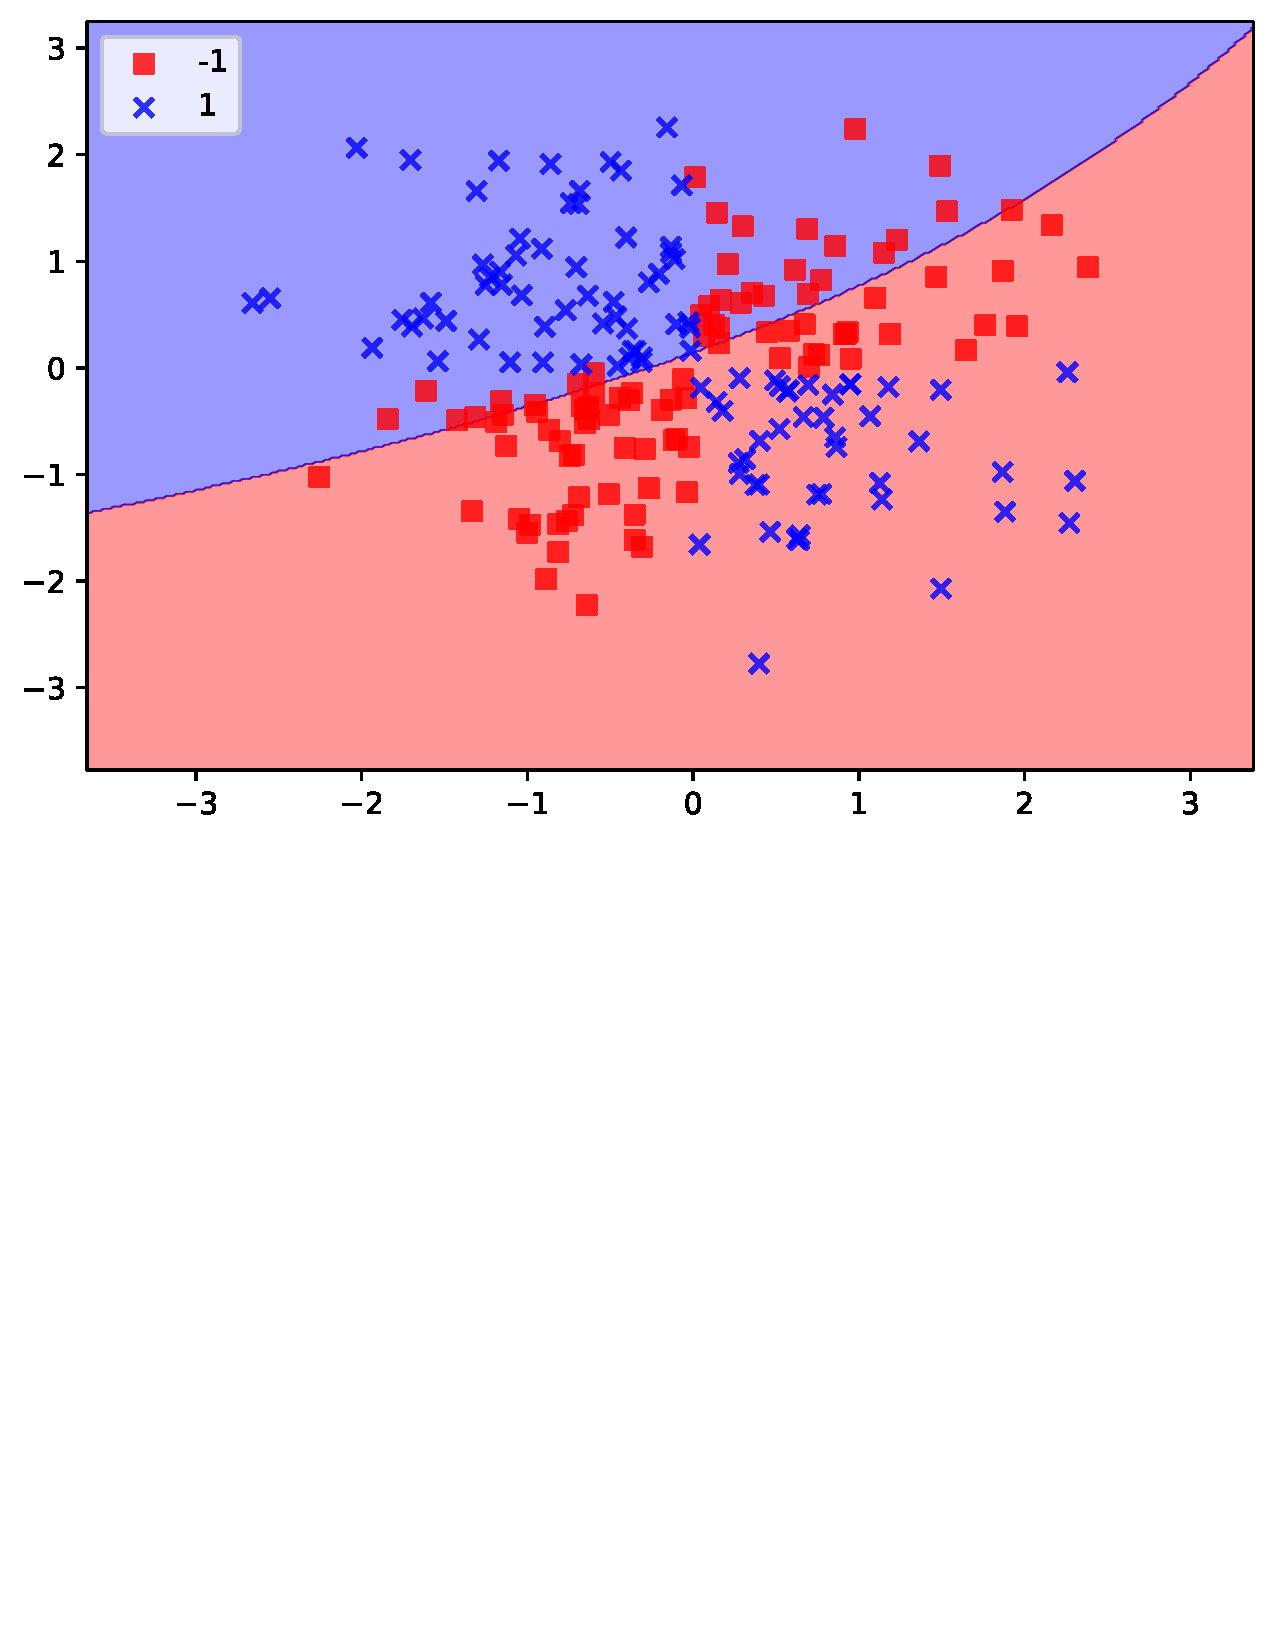
\includegraphics{figures/c-01.pdf}
          }
        }
      }
      \vspace{2.5cm}
      \only<2>{
        \makebox[\linewidth][c]{
          \resizebox{\linewidth}{!}{
            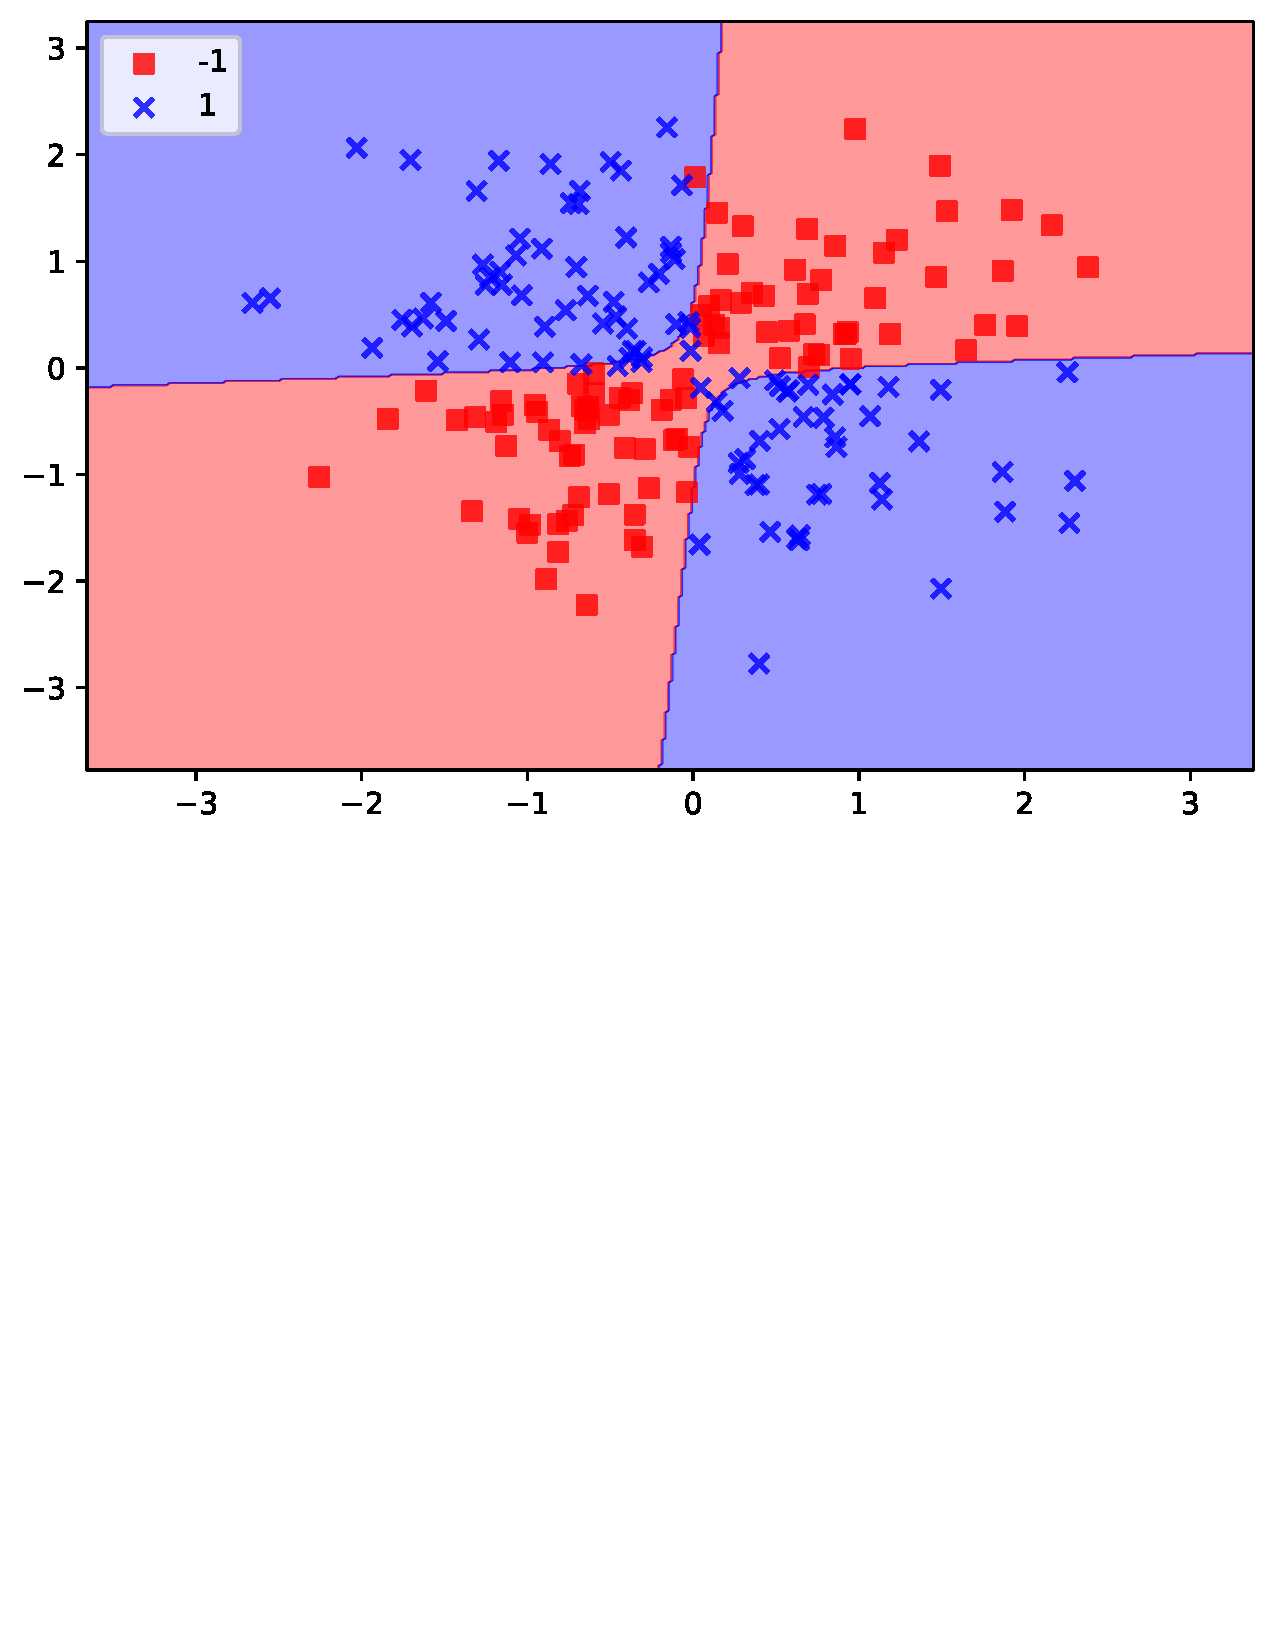
\includegraphics{figures/c-02.pdf}
          }
        }
      }
    \end{column}%
  \end{columns}
\end{frame}


% \begin{frame}[fragile]{\textbf{Q. SVM's C (regularization) hyperparameter?}}
%   \vspace{.4em}
%   \begin{wideitemize}
%   \item $C$ is the penalty for misclassifying data points:
%   \vspace{.4em}
%   \begin{wideitemize}
%   \item[-] When $C$ is small, the classifier is okay with misclassifying data
%     points; {\footnotesize if it's too small it can lead to underfitting (high bias, low variance)}.
%   \item[-] When $C$ is large, the classifier is heavily penalized for misclassifying
%     data points and therefore it bends over backwards avoiding any misclassified
%     data points; {\footnotesize if it's too large it can lead to overfitting (low bias, high variance)}.
%   \end{wideitemize}
%   \end{wideitemize}
% \end{frame}

\begin{frame}[fragile]{\textbf{Q. SVM's $\gamma$ hyperparameter (of Radial Basis
      Function (RBF) Kernel)?}}
  \begin{columns}[T] % align columns
    \begin{column}{.7\textwidth}
      \begin{wideitemize}
      \item $\gamma$ (\textit{Gamma}) is the ``spread'' of the RBF kernel $\&$
        hence the decision region.
        \begin{wideitemize}
        \item[-]<1-> When $\gamma$ is low, the ``curve'' of the decision boundary is very
          low (like an arch) and thus the decision region is very broad.
        \item[-]<2-> When $\gamma$ is high, the ``curve'' of the decision boundary is
          high; meaning the decision boundary mostly depends on individual data
          points, creating islands of decision-boundaries around data points (may overfit).
        \end{wideitemize}
      \end{wideitemize}
    \end{column}%
    \hfill%
    \begin{column}{.28\textwidth}
      \only<1>{
        \makebox[\linewidth][c]{
          \resizebox{\linewidth}{!}{
            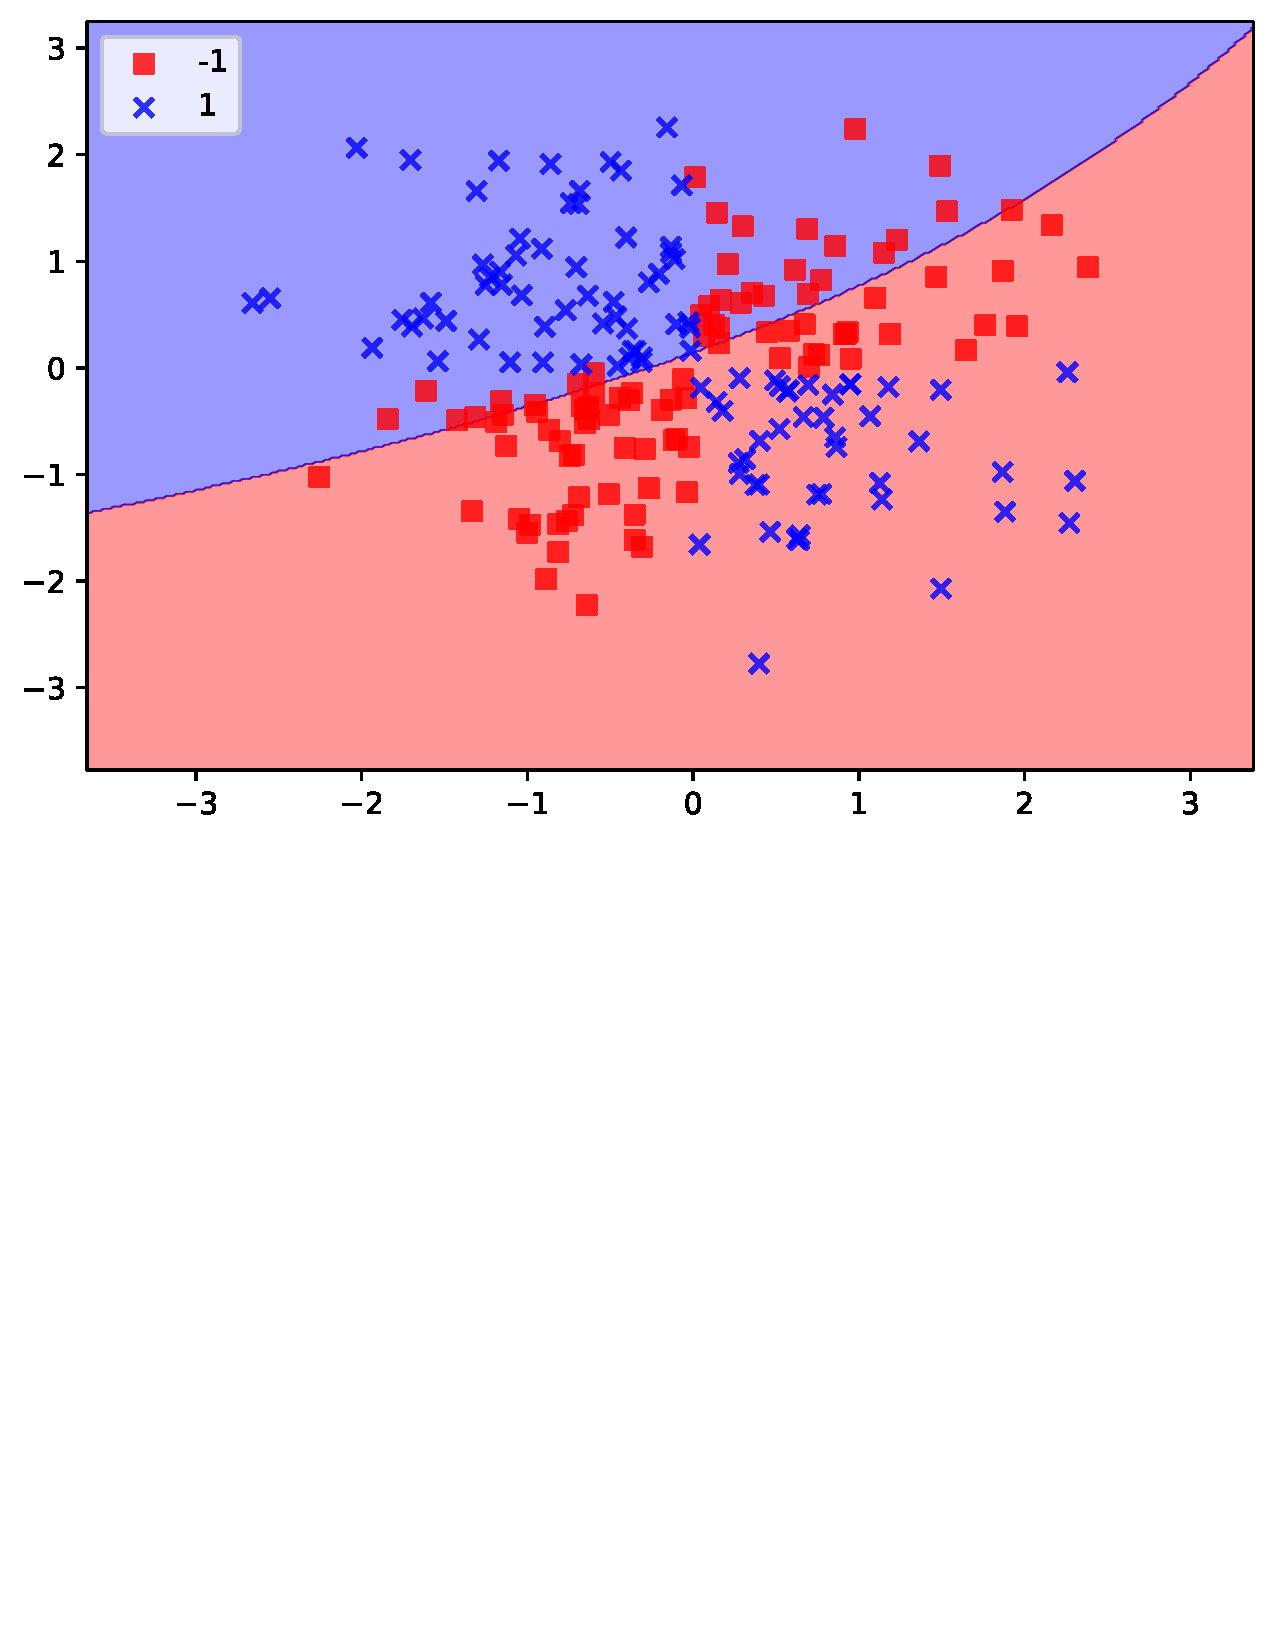
\includegraphics{figures/gamma-01.pdf}
          }
        }
      }
      \vspace{3cm}
      \only<2>{
        \makebox[\linewidth][c]{
          \resizebox{\linewidth}{!}{
            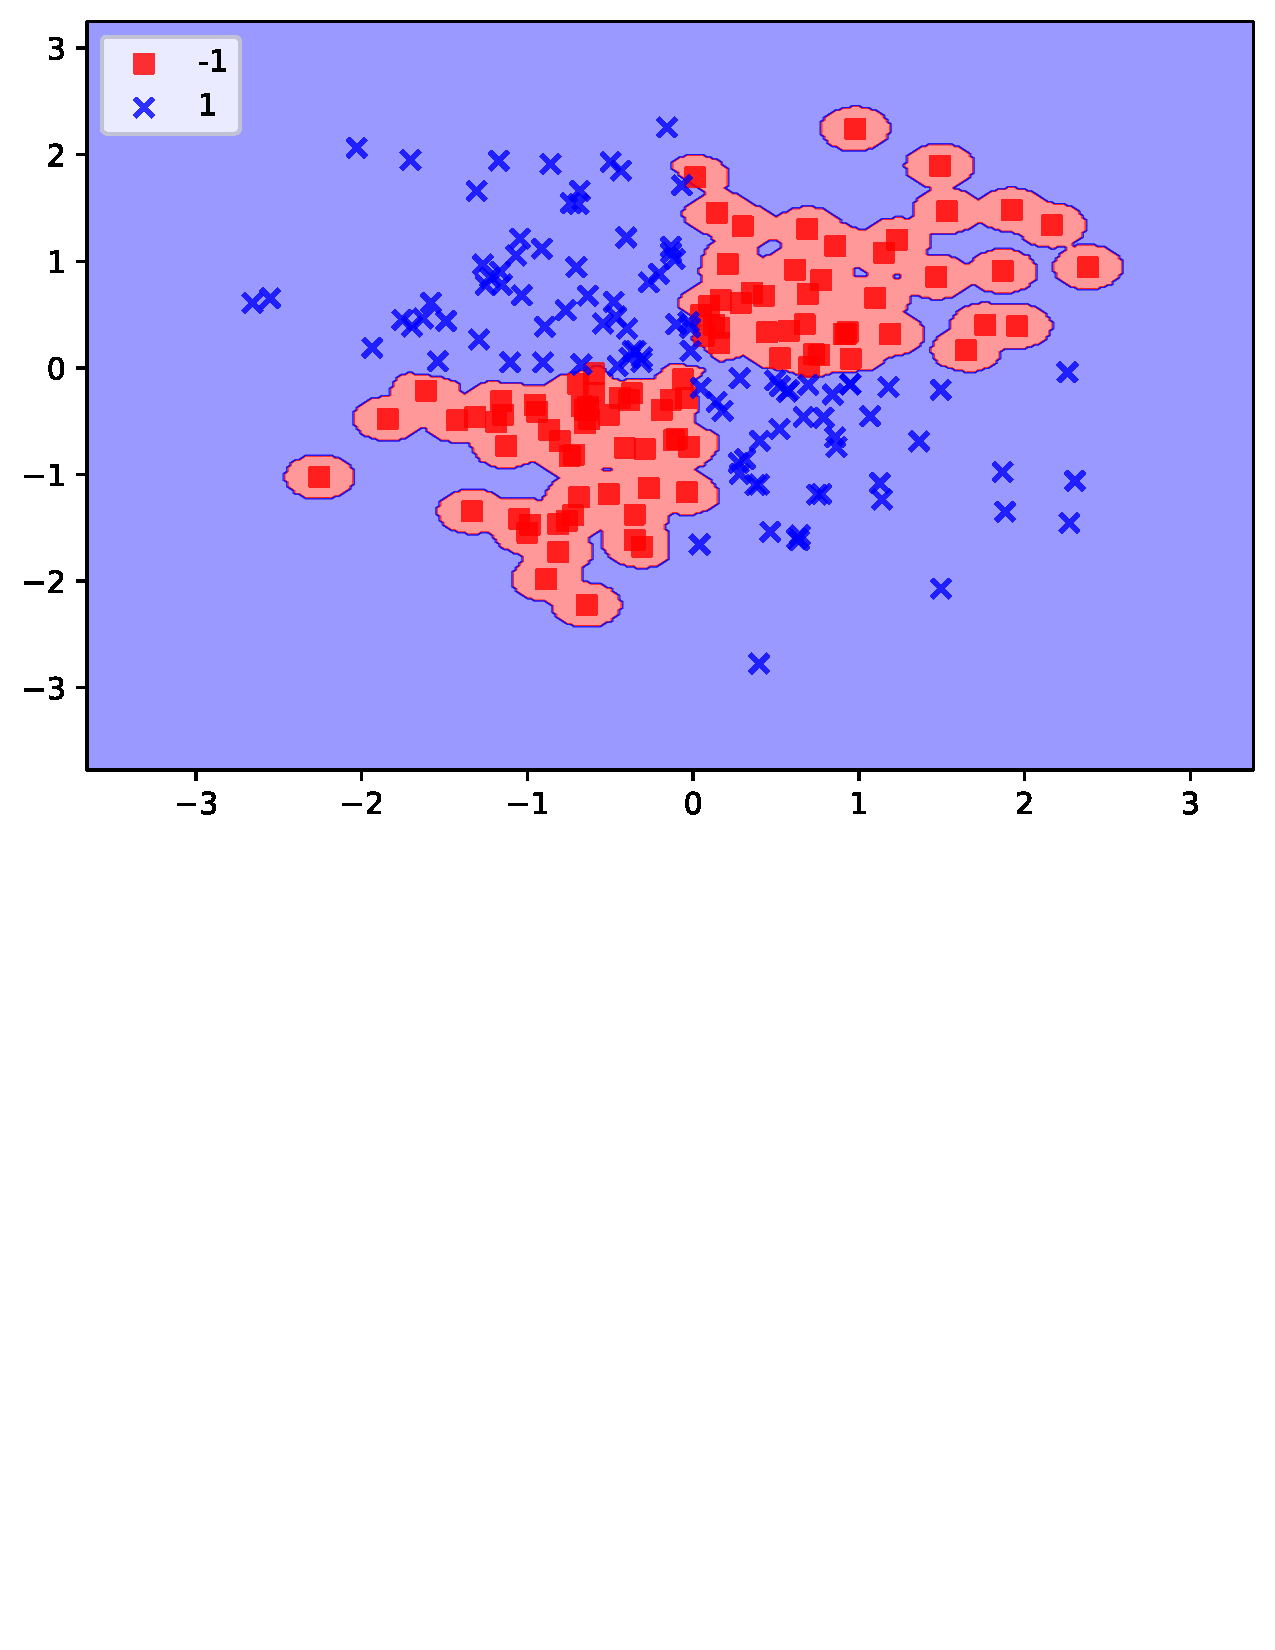
\includegraphics{figures/gamma-02.pdf}
          }
        }
      }
    \end{column}%
  \end{columns}
\end{frame}

% \begin{frame}[fragile]{\textbf{Q. SVM's $\gamma$ hyperparameter (of Radial Basis
%       Function (RBF) Kernel)?}}
%   \vspace{.4em}
%   \begin{wideitemize}
%   \item $\gamma$ (\textit{Gamma}) is the ``spread'' of the RBF kernel $\&$ hence the decision region.
%     \begin{wideitemize}
%     \item[-] When $\gamma$ is low, the ``curve'' of the decision boundary is very
%       low (like an arch) and thus the decision region is very broad.
%     \item[-] When $\gamma$ is high, the ``curve'' of the decision boundary is
%       high; meaning the decision boundary mostly depends on individual data
%       points, creating islands of decision-boundaries around data points (may overfit).
%     \end{wideitemize}
%   \end{wideitemize}
% \end{frame}


\begin{frame}[fragile]{\textbf{Q. What is Unsupervised Learning?}}
  \begin{wideitemize}
    \item In \textbf{Unsupervised Learning} (or \textbf{UL}), you are given a
    bunch of data and you are not told they fall naturally into clusters, and
    also you are not told what these clusters are.
    \item \textcolor{blue}{The goal is identify the clusters within data, how
    many clusters there are, and then be able to assign new things to
    these different clusters.}
  \end{wideitemize}
\end{frame}


\begin{frame}[fragile]{\textbf{Q. Examples of unsupervised learning?}}
  \begin{wideitemize}
  \item \textbf{Learning associations}\vspace{.4em}
    \begin{wideitemize}
    \item[-] Basket analysis. Let $\Pr(Y \mid X)$ the probability that a
      customer who buys $X$ also buys $Y$ -- estimated from past purchases. If
      $\Pr(Y \mid X)$ is $0.7$ then associate X to Y ($X \rightarrow Y$);
      meaning when someone buys $X$, recommend $Y$.
    \end{wideitemize}
  \item \textbf{Clustering} (group similar data points).
  \item \textbf{Density estimation} (where are data points likely to lie?)
  \item \textbf{Feature selection} (keep only useful features).
  \item \textbf{Outlier/novelty detection}.
  \end{wideitemize}
\end{frame}

\begin{frame}[fragile]{\textbf{Q. Can you give an example of Unsupervised Learning?}}
  \begin{wideitemize}
  \item \textcolor{blue}{Principal Component Analysis (or \textbf{PCA})}. In
    general terms, PCA is about finding the underlying patterns of the data and
    also gives you a method for data compression.\medskip
    \begin{wideitemize}
    \item If you want to \textit{approximate}\footnote{All your vectors can be
        written as the sum of a few $w$s.} the whole matrix with few vectors,
      the best vectors to choose are top PCA vectors (the principal components).
    \end{wideitemize}
  \item PCA is all about diagonalizing the covariance matrix.
    \begin{wideitemize}
    \item PCA is an exercise in linear algebra on very high dimensional vector spaces.
    \end{wideitemize}
  \end{wideitemize}
\end{frame}


\note[itemize]{
\item SVD vs PCA: SVD allows us to extract and untangle information, decompose a
  matrix into several component matrices (factorization), meaning it exposes many
  of the useful and interesting properties of the original matrix.  PCA can be
  computed form SVD but that will be much more expensive.
}


\begin{frame}[fragile]{\textbf{Q. Unpacking PCA?}}
  \begin{wideitemize}
    \item \textcolor{blue}{Principal Component Analysis (or \textbf{PCA})} is a classical UL algorithm.
    \item In \textbf{PCA}, the way this works, we construct a \textit{covariance matrix},
    and my covariance matrix is just the following object: $C = \sum_{j} \vec{v}_j\vec{v}^{\dagger}_{j}$,
    where $\vec{v}^{T}_{j}$ is the transpose of $\vec{v}_{j}$.
    \begin{wideitemize}
      \item[-] In other words, we construct $C$ from the data by taking these vectors $\vec{v}_j$ and
      multiply them by their transpose $\vec{v}^{\dagger}_j$.
      %\item E.g., Financial forecasting: the vectors could be, for example, can
      %represent the changes in stock prices over a 24 hr period, and the
      %covariance matrix $C$ would give the correlations (or covariances in the
      %data) between the prices of the different stocks in different times within
      %the 24 hrs period.
    \end{wideitemize}
    \item In \textbf{PCA}, you diagonalize $C$ and say $C = \sum_{k} P_k
	  \vec{\omega}_{k}\vec{\omega}^{\dagger}_{k}$\footnote{C can be decomposed into a product
    of matrices involving eigenvalues and eigenvectors}, $P_k$ is piece of the data with size $k$,
    and $\vec{\omega}_{k}$ are the set of vectors you need to find.
    \item If and only if a small set of $P_k >> 0$, then $C$ is effectively low-rank,
    and the corresponding $\vec{\omega}_{k}$ are the principal components. In other words,
    you need find the eigenvectors that have the largest eigenvalues -- i.e., your principal components.
  \end{wideitemize}

\end{frame}


\begin{frame}[fragile]{\textbf{Q. When to use PCA?}}
  \vspace{.4em}
  \begin{wideitemize}
    \item \textbf{When to use it}
    \begin{wideitemize}
      \item PCA should be used if one to figure out if there are latent features
      driving the patterns in the data. E.g., The big shots at SRI International.
      \item Dimensionality reduction (and feature selection). E.g., helps you
      visualize high dimensional data, helps you reduce noise in your data, make
      other ML algos work better (regression, classification) because fewer inputs.
    \end{wideitemize}
    \item \textbf{When not to use it}
    \begin{wideitemize}
      \item PCA is not suitable in many cases: For example, if all the components of PCA
      have quite a high variance, there is no \textit{good} universal stopping rule that
      allows you to discard some exact \textit{k} Principal Components, meaning no good
      data compression.
      \item Not good when working with fine-grained classes\footnote{hard-to-distinguish object classes}.
    \end{wideitemize}
  \end{wideitemize}
\end{frame}

% \begin{frame}[fragile]{\textbf{Q. Recap: Advantages and Disadvantages of PCA?}}
%   \vspace{.4em}
%   \begin{wideitemize}
%     \item \textbf{Advantages}
%     \begin{wideitemize}
%       \item Dimensionality reduction
%       \item Allows estimation of probabilities in high-dimensional data.
%       \item It renders a set of components that are uncorrelated (latent features).
%     \end{wideitemize}
%     \item \textbf{Disadvantages}
%     \begin{wideitemize}
%       \item It has a high computational cost, meaning it'll struggle with very large datasets.
%       \item Non-linear structure is hard to model with PCA.
%     \end{wideitemize}
%   \end{wideitemize}
% \end{frame}

\begin{frame}[fragile]{\textbf{Q. What is Reinforcement Learning?}}
  \begin{wideitemize}
    \item Reinforcement learning is one of three basic machine learning paradigms, alongside
    supervised learning and unsupervised learning.
    \item In reinforcement learning an algorithm learns to do something by being
    rewarded for successful behavior and/or being punished for unsuccessful
    behavior. {\footnotesize No supervised output but delayed reward.
      \textbf{Ex:} playing chess or a computer game, robot in a maze.}
  \end{wideitemize}
\end{frame}

\note[itemize]{
\item In a supervised learning model, the algorithm learns on a labeled
dataset, providing an answer key that the algorithm can use to evaluate its
accuracy on training data.
\item An unsupervised model, in contrast, provides unlabeled data that the
algorithm tries to make sense of by extracting features and patterns on its own.
}

\begin{frame}[fragile]{\textbf{Q. Can you give an example of Reinforcement Learning?}}
  \begin{wideitemize}
    \item Policy Gradient (PG)
    \begin{wideitemize}
      \item In this method, we have the policy $\pi$ that has a parameter $\theta$. This $\pi$
      outputs a probability distribution of actions.
      \item Then we must find the best parameters ($\theta$) to maximize (optimize) a score
      function $J(\theta)$, given the discount factor $\gamma$ and the reward $r.$
      \item Main steps:\medskip
      \begin{wideitemize}
        \item Measure the quality of a policy with the policy score function
        \item Use policy gradient ascent to find the best param that improves the policy.
      \end{wideitemize}
    \end{wideitemize}
  \end{wideitemize}
\end{frame}

% \subsection{Machine Learning problems}
% \begin{transitionsubframe}
%   \begin{center}
%     \Huge Examples of Classification and Regression problems
%   \end{center}
% \end{transitionsubframe}


% \begin{frame}[fragile]{\textbf{Q. Can you give an example of a Classification Problem?}}
%   \begin{wideitemize}
%     \item E.g., trying to write a machine learning program that will be able to detect cancerous
%     tumors in lungs. It takes in images of lung x-rays as input and determines if there is a tumor.
%     If there is a tumor, we'd like the computer to output ``yes'' and if there is not a tumor, we'd
%     like the computer to output ``no.'' We’d like the computer to output the correct answer as much as possible.
%     \item Say the training set for this algorithm consists of several images of x-rays, half of the images
%     contain tumors and are labelled ``yes'' and the other half do not contain tumors and are labelled ``no.''
%   \end{wideitemize}
% \end{frame}

% \begin{frame}[fragile]{\textbf{Q. Can you give an example of a Regression Problem?}}
%   \begin{wideitemize}
%     \item In regression problem the goal of the algorithm is to predict real-valued output.
%     \item E.g., Let’s consider the problem of predicting the marks of a student based on the number of hours he/she
%     put for the preparation.
%     \begin{wideitemize}
%       \item Assume for the sake of understanding that the marks of a student (M) do depend on the number of hours (H) he/she put up for preparation.
%       \item The following formula can represent the model: $M = m*H + c$
%     \end{wideitemize}
%   \end{wideitemize}
% \end{frame}

% \begin{frame}[fragile]{\textbf{Q. Classification vs Regression?}}
%   \begin{wideitemize}
%     \item Classification is the task of predicting a discrete class label.
%     \item Regression is the task of predicting a continuous quantity.
%     \item There's some overlap between classification and regression algorithms; for example
%     \begin{wideitemize}
%       \item A classification algorithm may predict a continuous value, but the continuous value is in the form of a probability for a class label.
%       \item A regression algorithm may predict a discrete value, but the discrete value in the form of an integer quantity.
%     \end{wideitemize}
%   \end{wideitemize}
% \end{frame}


\subsection{Data representation}
\begin{transitionsubframe}
  \begin{center}
    \Huge Data representation
  \end{center}
\end{transitionsubframe}

\begin{frame}[fragile]{\textbf{Q. How do you represent data in ML?}}
  \begin{wideitemize}
    \item In general, the given data is expressed in a form of a bunch of vectors
    $\vec{v}_{j} \in {\Bbb R}^{d}$ that belong to some high dimensional vector space.
    \item For instance, in image recognition, the vector\footnote{a.k.a., feature
    vector; it could be numerical (e.g., height of tree) or descriptive
    (e.g., eye color)} of an each image is a set of pixels\footnote{each entry
    in the vector (e.g., pixel) represents a feature.} (i.e., a pixelated
    version of the image).
    \item If you have a notion of distance $\Delta(\vec{v}_{i}, \vec{v}_{j})$,
    then you can compare which vectors are close to each other in this high
    dimensional vector space; e.g., the norm $\norm{\vec{v}_{i} - \vec{v}_{j}}^2$.
  \end{wideitemize}
\end{frame}

\begin{frame}[fragile, label={distance}]{\textbf{Q. What is it important about measuring distances?}}
  \begin{wideitemize}
    \item Because the shorter the distance between two feature vectors the closer
    in character are the two samples they represent.
    \item There are many ways to measure distance:
    \begin{wideitemize}
      \item[-] \textbf{Manhattan distance} ($L^{1}$ norm). The sum of the absolute values of the different between
      entries in the vector. {\footnotesize (Preferred dist. when dealing with high dimensional data.)}
      \item[-] \textbf{Euclidean distance} ($L^{2}$ norm). Square the distances between vector entries,
      sum these and square root.
      \item[-] \textbf{Cosine similarity}. Cosine of the angle between two vectors\footnote{Two vectors
      might be similar if they are pointing in the same direction even if they are of different lengths.}.
      Just take the \textit{dot} product of two vectors and divide by the two lengths.
    \end{wideitemize}
  \end{wideitemize}
\end{frame}

\begin{frame}[fragile, label={CoD}]{\textbf{Q. Any other issues we should care to learn?}}
  \begin{wideitemize}
    \item The curse of dimensionality. This phenomena involves data in high dimensions.
    \item \textbf{Ex}. Suppose you are working in $M$ dimensions, that is you data has $M$
    features. And suppose you have $N$ data points. Having a large number of
    data points is good, the more the merrier. BUT what about number of features?
    \item Think how these $N$ data points might be distributed over $M$ dimensions.
    Suppose that the numerical data for each feature is $0$ or $1$. Therefore, there
    will be $2^{M}$ possible combinations.
   \item {\footnotesize If $N$ is less than $2^{M}$ then you run the risk of
      having every data point being on a different corner of the $M$-dimensional hypercube.}
  \end{wideitemize}
\end{frame}

\subsection{Process overview}
\begin{transitionsubframe}
  \begin{center}
    \Huge Building a Machine learning model
  \end{center}
\end{transitionsubframe}

\begin{frame}[fragile]{\textbf{Q. What does this process looks like?}}
  \begin{wideitemize}
    \item \textbf{Explore and clean the data}. Explore the data to really understand
    what those features look like, then we use some of these learnings to clean the data.
    \item \textbf{Split data into train/validation/test data sets}.
    \item \textbf{Fit an initial model (baseline) and evaluate using 5-fold cross-validation}.
    % We will use 5-fold cross
    % validation o the training set to fit an initial model to see what we can expect
    % for the baseline performance of the model.
    \item \textbf{Tune hyper-parameters using GridSearchCV} to find the best models\footnote{those models that beat our baseline}.
    \item \textbf{Evaluate best models on validation set} and select the top model of each
    algorithm, and we evaluate them against each other on the validation set.
    \item \textbf{Select and evaluate the final model on the test set}. We'll evaluate top
    model on the test set to get an unbiased view of the model performance on completely unseen data.
  \end{wideitemize}
\end{frame}

\section{Measuring success}
\begin{transitionframe}
  \begin{center}
    \Huge Measuring success
  \end{center}
\end{transitionframe}

\begin{frame}[fragile, label={distance}]{\textbf{Q. What does it mean to measure success of the model?}}
  \begin{wideitemize}
    \item So the question is how do we make sure the model is learning the underlying pattern
    and not just memorizing the examples?
    \item We can do this by splitting our data into three data sets: the training, validation,
    and testing data sets.\medskip
    \begin{wideitemize}
      % \item[-] This part is about the model needing to learn the underlying pattern
      % (or correlation) that will allow it to make predictions about future examples.
      % The first step is walking through why it's necessary to split up our data before
      % we build a model. Please recall the definition of ML that we settled on back in the first
      % section of these slides. Particularly, recall the part on generalizing to make predictions
      % about new examples. This part is about the model needing to learn the underlying pattern
      % (or correlation) that will allow it to make predictions about future examples.
      \item This part is about making sure the model is learn the underlying pattern
      (or correlation) and able to make predictions about future examples.
    \end{wideitemize}
  \end{wideitemize}
\end{frame}

\note[itemize]{
\item Now that we have a decent idea of how to explore and clean our data, we want to start
setting the stage for building a model by understanding what it means to measure success of
the model.
}


\begin{frame}[fragile]{\textbf{Q. But why do we split the data?}}
  \begin{wideitemize}
    \item \textbf{Ans.} We do it to make sure\footnote{We don't know how well the model will generalize
    because we don't have any additional data to test this.} our model is learning
    the underlying pattern and not just memorizing the examples.
    \item We do that by splitting our dataset into three separate segments;
    training (60\%), validation (20\%), and testing (20\%) data sets.\medskip
    \begin{wideitemize}
      \item \textbf{Training data}, or examples that the model will learn
      those general patterns from.
      \item \textbf{Validation data}, or examples we use to select the best model (optimal algorithm
      and hyper-parameter settings).
      \item \textbf{Test data}, or examples we use to provide an unbiased evaluation of what
      the model will look like in its real environment.
    \end{wideitemize}
  \end{wideitemize}
\end{frame}


\begin{frame}[fragile]{\textbf{Q. Why does the evaluation process look like with these datasets?}}
  \begin{wideitemize}
    \item[1.] You start train your ML algorithm on the training data, evaluate it
    using the validation data, then at this point:\medskip
    \begin{wideitemize}
      \item If none of your models are any good based on the performance on the
      validation set, then you need to revisit the training phase and consider
      some new variables or new models. (Go back to step 1.)
      \item If the performance is quite good, then you can select your best model
      and pass it onto the testing phase. (Go to step 2.)
    \end{wideitemize}
    \item[2.] You evaluate the best model on the test set.\medskip
    \begin{wideitemize}
      \item If the performance is what you expect, then that model is ready to go.
      Otherwise go to step to the drawing board.
    \end{wideitemize}
  \end{wideitemize}
\end{frame}

\begin{frame}[fragile]{\textbf{Q. What is cross-validation? Holdout test set?}}
  \begin{wideitemize}
    \item \textbf{Holdout test set:} A generalization of the test set. It's just any data set
    that was not used in fitting a model (data set aside for evaluating the model's ability to generalize).
    \item \textbf{K-Fold Cross-Validation:} Data is divided into $k$ subsets and the holdout method
    is repeated $k$ times. Each time, one of the $k$ subsets is used as the test set and the other
    $k - 1$ subsets are combined to be used to train the model.
  \end{wideitemize}
\end{frame}

\note[itemize]{
\item The previous process how to use training, validation and test set to measure
our model's ability to generalize.
}

\begin{frame}[fragile]{\textbf{Q. 5-Fold Cross-Validation Example?}}
  \begin{wideitemize}
    \item E.g., $5$-fold CV: Given $10,000$ examples, you partition into $5$ buckets, each consisting
    of $2,000$ examples\footnote{this is partitioning is done thru sampling without replacement; no
    single example will appear in two different subsets and all original $10,000$ are still
    accounted for in these subsets}.
    \item \textbf{On trial} $1$, we set aside the last bucket (holdout test set) and the other $4$ buckets are the
    training set, then compute its predictive performance. On \textbf{trial} $2$, we set aside the penultimate
    bucket, and the other $4$ buckets are the training set. This will be similar for the other $3$ \textbf{trials}.
    \item At the end we \textit{average} the performance of model over the many trails.
  \end{wideitemize}
\end{frame}

\begin{frame}[fragile]{\textbf{Q. Establishing our Evaluation framework?}}
  \begin{wideitemize}
    \item A cohesive framework for evaluating our model, consisting of two components:\medskip
    \begin{wideitemize}
      \item \textbf{Evaluation metrics}: how are gauging the accuracy of the model?
      \item \textbf{Process (how to split the data)}: how do we leverage a given
      data set to mitigate the likelihood of overfitting and underfitting.
    \end{wideitemize}
  \end{wideitemize}
\end{frame}

\subsection{Evaluation metrics}
\begin{transitionsubframe}
  \begin{center}
    \Huge Evaluation metrics:\\\textbf{There isn't a one-size-fits-all metric.}
  \end{center}
\end{transitionsubframe}

\begin{frame}[fragile]{\textbf{Q. What are the evaluation metrics that we'll use?}}
\begin{wideitemize}
  \item The metric(s) chosen to evaluate a ML model depends on various factors:\medskip
  \begin{wideitemize}
    \item Is it a regression or a classification task? E.g., MSE vs Accuracy.
    \item What is the business objective? E.g., precision vs recall.
    \item What is the distribution of the target variable?
  \end{wideitemize}
  \item Examples of other metrics: Mean Absolute Error (MAE), Mean Squared Error
    (MSE), R-squared, Confusion Matrix and related metrics (Precision, Recall, Accuracy).
\end{wideitemize}
\end{frame}

\note[itemize]{
\item Regression: Mean Squared Percentage Error (MSPE), Mean Absolute Error (MAE),
Minimum Sum of Absolute Error (MSAE), Mean Squared Error (MSE), R-squared, Adjusted R-squared
\item Classification: Confusion Matrix and related metrics (Precision, Recall, Accuracy),
Receiver Operating Characteristics \& Area under the curve (ROC-AUC), log-loss, F1-score
}


\begin{frame}[fragile]{\textbf{Q. Measuring classifier performance?}}
  \begin{wideitemize}
  \item Binary classification:\medskip
    \begin{wideitemize}
    \item Accuracy\footnote{or classification error: \textit{\#(misclassified) /
          \#(total examples)} ($1$ - Accuracy)} in \%: \textit{\#(classified correctly) / \#(total examples)}
    \item Precision: \textit{\#(classified correctly as A) / \#(total examples
        predicted in A)}
    \item Recall: \textit{\#(classified correctly as A) / \#(total examples
        known in A)}. {\footnotesize We can always achieve perfect recall by
        returning the entire dataset (which will contain many irrelevant examples)}
    \end{wideitemize}
  \end{wideitemize}
\end{frame}



\begin{frame}[fragile]{\textbf{Q. Measuring classifier performance?}}
  \begin{wideitemize}
  \item Binary classification:\medskip
    \begin{wideitemize}
    \item Receiver operating curve (ROC): the pair values (false positive rate
      or FPR, true positive rate or TPR) as a function of a threshold $\theta \in [0, 1]$.
      {\footnotesize An ideal classifier is at $(0, 1)$ (top left corner). Diagonal ($FPR
        = TPR$): random classifier. \textit{This is the worst we can do}.}
      {\scriptsize Any classifier that is below the diagonal can be improved by flipping its decision.}
    \item Area under the curve (AUC): It reduces the ROC to a number. Ideal
      classifier: $AUC = 1$. {\footnotesize ROC and AUC allow us to compare
        classifiers over different loss conditions, and choose a value of
        $\theta$ accordingly. Often, there is not a dominant classifier.}
    \end{wideitemize}
  \end{wideitemize}
\end{frame}

\begin{frame}[fragile]{\textbf{Q. Measuring classifier performance?}}
  \begin{wideitemize}
  \item $K > 2$ classes:\medskip
    \begin{wideitemize}
    \item Again, the most basic measure is the classification error.
    \item \textit{Confusion matrix:} $\text{K}\times \text{ K}$ matrix where entry \textit{(i, j)} contains the
      number of instances of class $C_i$ that are classified as $C_j$.
    \item {\footnotesize It allows us to identify which types of misclassification errors tend
        to occur, e.g. if there are two classes that are frequently confused.
        \textbf{Ideal classifier:} the confusion matrix is diagonal.}
    \end{wideitemize}
  \end{wideitemize}
\end{frame}


\begin{frame}[fragile]{\textbf{Q. What is a confusion matrix?}}
  \begin{wideitemize}
  \item A \textbf{Confusion Matrix} is a simple way of understanding \textbf{how well an
      algorithm is doing at classifying data}. It is just the idea of \textbf{false
      positives} and \textbf{false negatives}
    \begin{flushleft}
      \makebox[\linewidth][l]{
        \resizebox{.60\linewidth}{!}{
          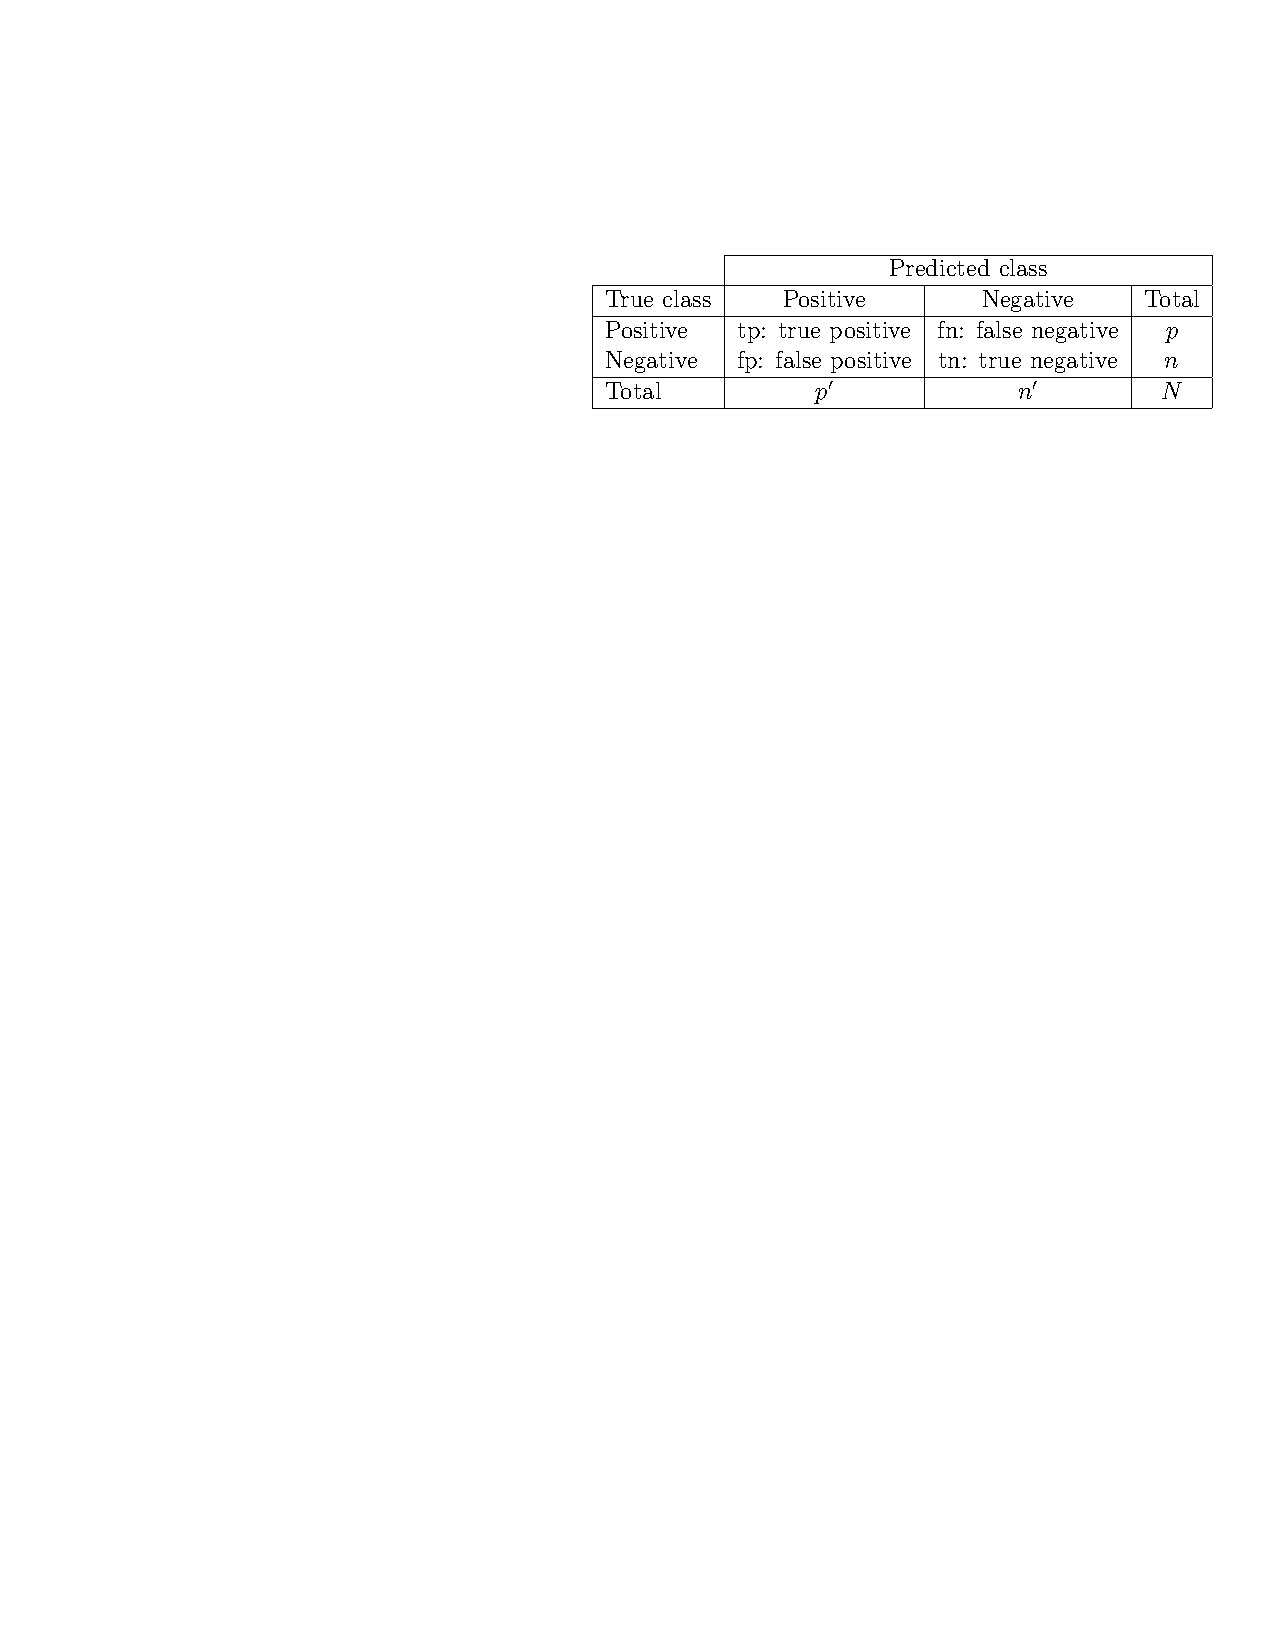
\includegraphics{figures/confusionmatrix.pdf}
        }
      }      
    \end{flushleft}
    % \item
    %   \begin{tabular}{cc|cc}
    %     \multicolumn{1}{c}{} &\multicolumn{1}{c}{} &\multicolumn{2}{c}{Predicted} \\
    %     \multicolumn{1}{c}{} & \multicolumn{1}{c|}{} & \multicolumn{1}{c}{Yes} & \multicolumn{1}{c}{No} \\ \hline
    %     \multirow[c]{2}{*}{\rotatebox[origin=tr]{90}{Actual}} & Yes & TP & FN \\[1.5ex] & No & FP & TN \\ \hline
    %   \end{tabular}
  \end{wideitemize}
\end{frame}

\begin{frame}[fragile]{\textbf{Q. Can you explain what precision and recall are?}}
\begin{wideitemize}
  \item \textbf{Recall} is a measure of completeness or quantity, whereas
   \item \textbf{Precision} is a measure of exactness or quality:\vspace{.4em}
  \begin{itemize}
    \item \parbox[t]{1.5in}{$\underbrace{Recall = \frac{TP}{TP +
            FN}}_{\substack{\text{What proportion of actual positives}\\ \text{was identified correctly?}}}$} \hspace{.6in}
      \parbox[t]{1.5in}{$\underbrace{Precision = \frac{TP}{TP + FP}}_{\substack{\text{What
            proportion of positive identifications}\\\text{was actually correct?}}}$}
  \end{itemize}
  \item \textbf{High precision} means your algorithm has returned
  substantially \textit{more relevant results than irrelevant ones}, while
  \textbf{high recall} means your algorithm has returned \textit{most of the
  relevant results}.
\end{wideitemize}
\end{frame}


\begin{frame}[fragile]{\textbf{Q. Can you explain what are false positives and false negatives?}}
  \begin{wideitemize}
  \item \textbf{False positives} and \textbf{false negatives}, technically
    referred to as type $I$ error and type $II$ error respectively.
  \item \textbf{False positives} are incorrect classifications of the presence
    of a condition when it is actually absent. {\footnotesize A \textbf{false positive} is \textcolor{red}{when you
      reject a true null hypothesis}}.
  \item \textbf{False negatives} are incorrect classifications of the absence of
    a condition when it is actually present. {\footnotesize A \textbf{false negative} is \textcolor{red}{when you accept
      a false null hypothesis}}.
  \end{wideitemize}
\end{frame}

\begin{frame}[fragile]{\textbf{Q. Provide examples when false positives are more
      important than false negatives, false negatives are more important than
      false positives and when these two types of errors are equally important}}
  \begin{wideitemize}
    \item Case 1, \textbf{Airport security}. Ensuring that truly dangerous items like
    weapons cannot be brought on board an aircraft. Getting false positives is better than
    getting false negatives: missing cases of actual weapons could lead to dangerous situations.
  \item Case 2, \textbf{Cancer screening}. Even though false-positive results could create
  anxiety and lead to unnecessary and invasive follow-up tests like biopsies, missing cases of
  actual cancer could lead to delays in treatment that negatively affect somebody's life.
  \item Case 3, \textbf{General forecasting} (health weather). Measuring success of testing cases
  of covid-19 in the US. Tracking rate of false positives and false negatives seems to make sense.
  \end{wideitemize}
\end{frame}

\begin{frame}[fragile]{\textbf{Q. Can you list other metrics derived from the Confusion Matrix?}}
  \begin{wideitemize}
  \item Confusion matrix related metrics (where $N$ is $TP + TN + FP + FN$)\\
    \begin{flushleft}
      \makebox[\linewidth][l]{
        \resizebox{.60\linewidth}{!}{
          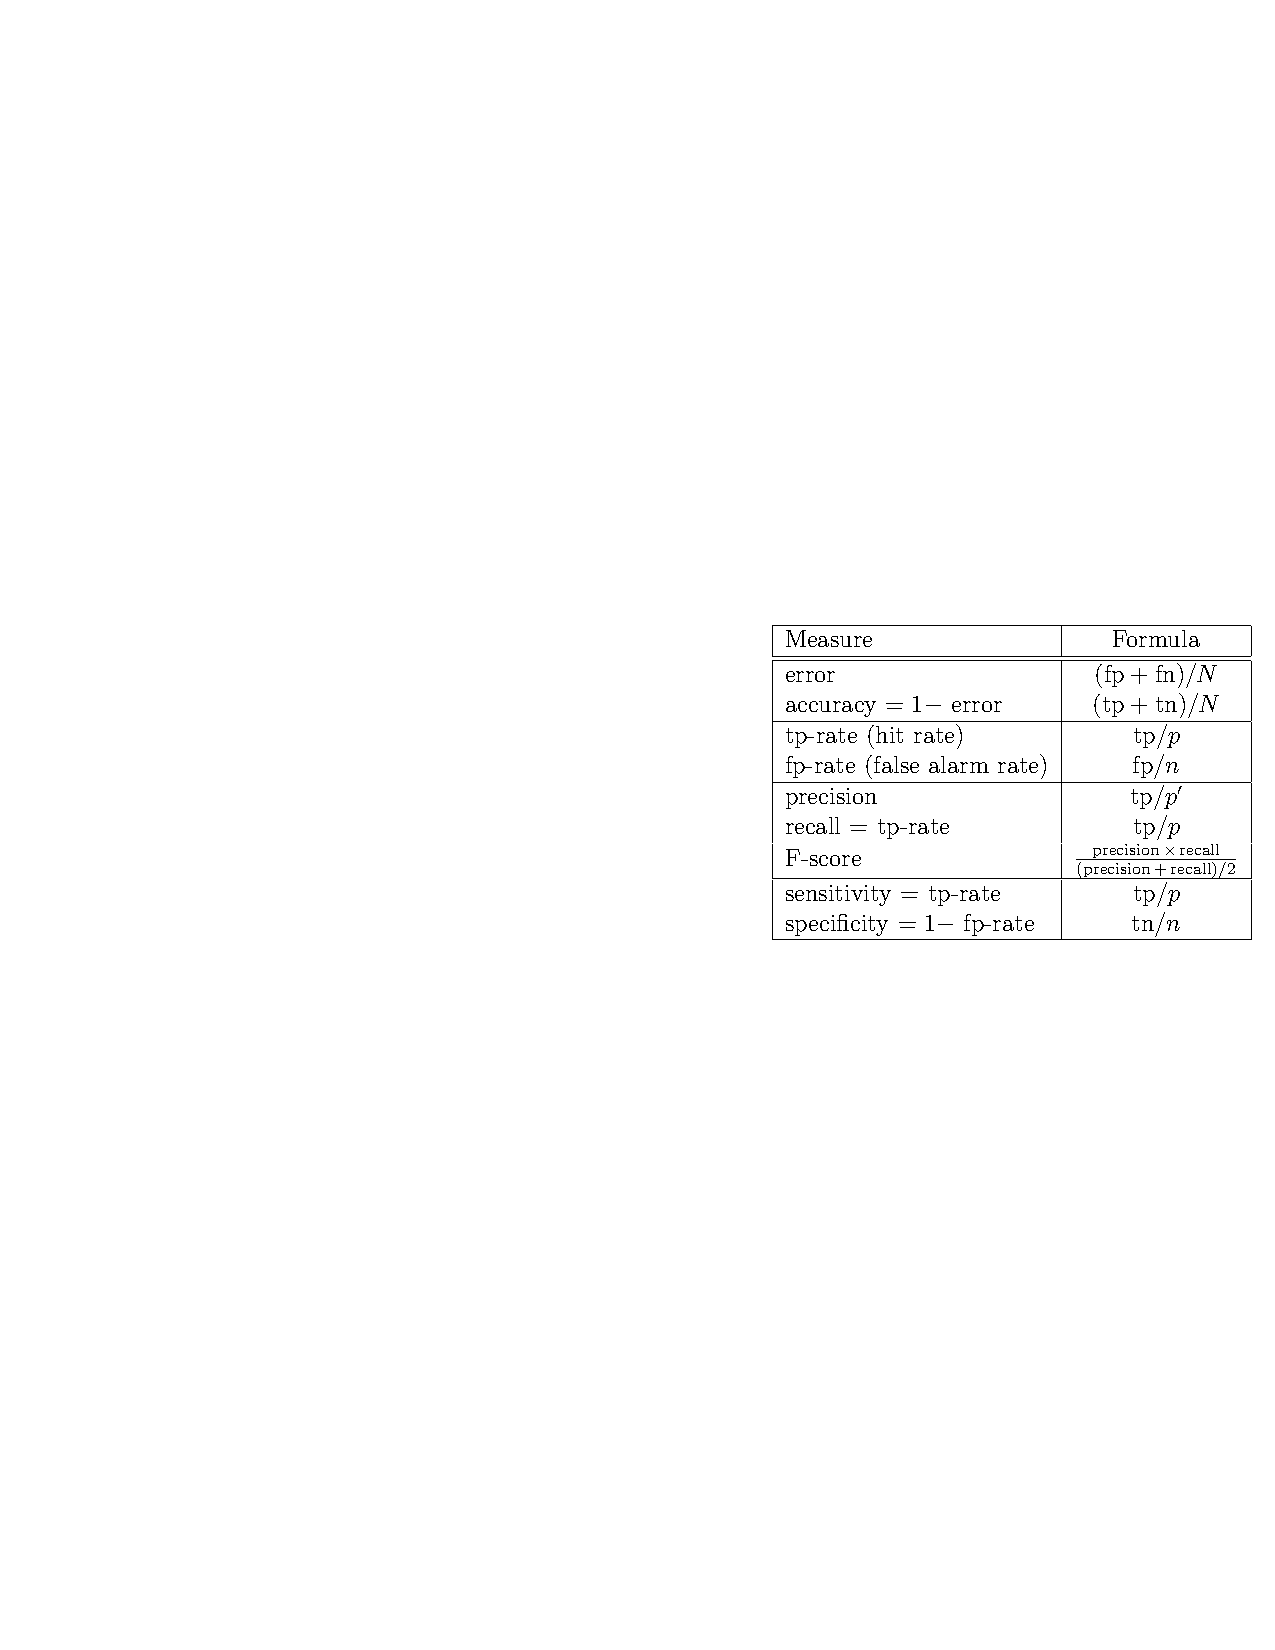
\includegraphics{figures/confusionmatrixmetrics.pdf}
        }
      }      
    \end{flushleft}
    % \begin{wideitemize}
    % \item Accuracy rate: {\footnotesize $\frac{TP + TN}{Total}$}
    %   where {\footnotesize Total is $TP + TN + FP + FN$},\vspace{-.5em}
    % \item Error rate: {\footnotesize $1 - \frac{TP + TN}{Total}$},\vspace{-.5em}
    % \item False positive rate\footnote{It's a measure of accuracy for a test}:
    % {\footnotesize $\frac{FP}{TN + FP}$},\vspace{-.5em}
    % \item False negative rate\footnote{It's proportion of the individuals with a known
    % positive condition for which the test result is negative}:
    % {\footnotesize $\frac{FN}{TP + FN}$},\vspace{-.5em}
    % \item Recall: {\footnotesize $\frac{TP}{TP + TN}$}, Precision: {\footnotesize $\frac{TP}{TP + FP}$},\vspace{-.5em}
    % \item Specificity: {\footnotesize $1 - \frac{FP}{TN + FP}$},\vspace{-.5em}
    % \item Prevalence: {\footnotesize $\frac{TP + FN}{Total}$}
    % \end{wideitemize}
  \end{wideitemize}
\end{frame}

\begin{frame}[fragile]{\textbf{Q. How do you measure how  good your
      classification algorithm is? You have unbalanced numbers, with our class
      being much larger or smaller than others}}
  \begin{wideitemize}
  \item You use the Matthews correlation coefficient. The number it yields is
    between plus or minus one. Plus one means perfect prediction, zero means no
    better than random.
  \item $\frac{\text{TP x TN - FP x FN}}{\sqrt{(TP + FP)(TP + FN)(TN + FP)(TN + FN)}}$
  \end{wideitemize}
\end{frame}


\begin{frame}[fragile]{\textbf{Q. ROC and AUC? Also given an example}}
  \begin{wideitemize}
  % \item Another way of looking at how well an algorithm is classifying is the
  %   \textbf{receiver operating characteristic} or \textbf{ROC} curve.
    \item E.g., suppose there is a threshold (or parameter) in your
      classification algorithm that determines whether you have an apple or a
      non apple object:\\
      \begin{flushleft}
        \makebox[\linewidth][l]{
          \resizebox{.60\linewidth}{!}{
            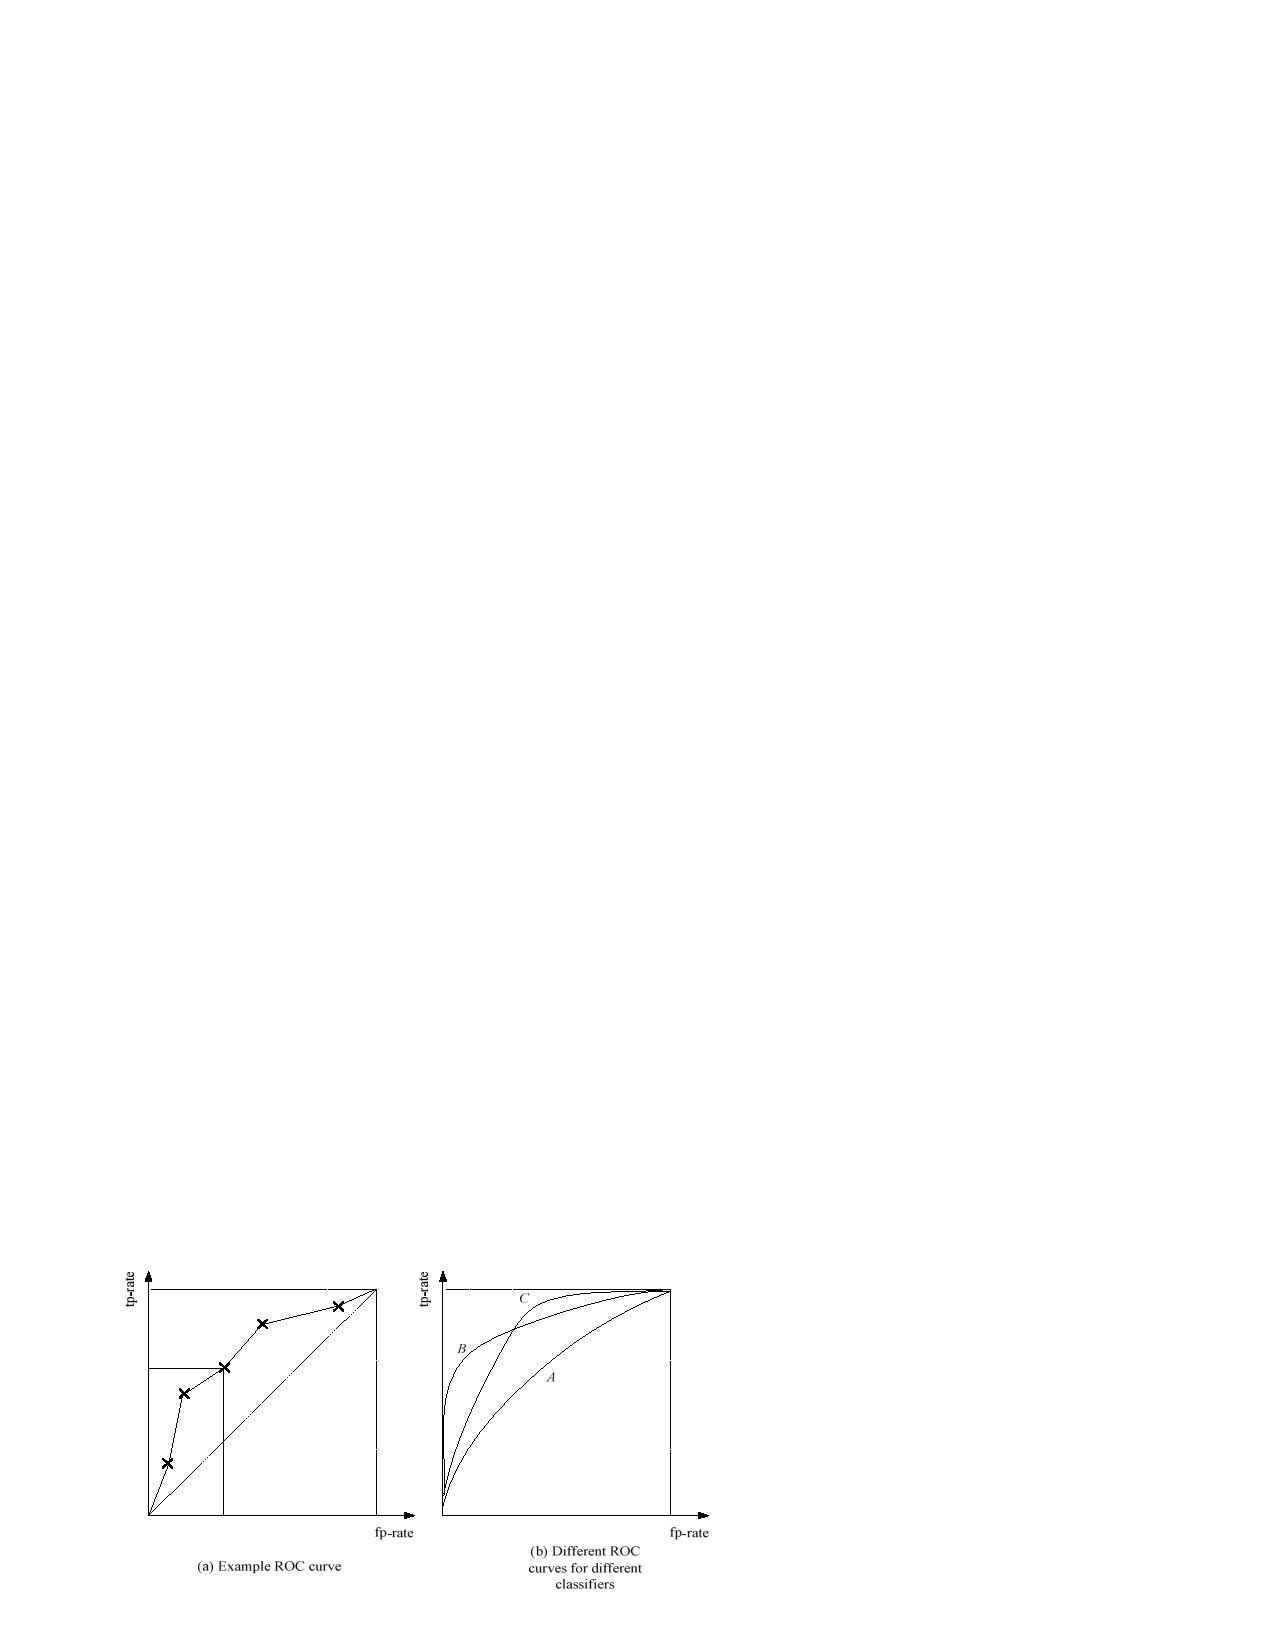
\includegraphics{figures/rocauc.pdf}
          }
        }      
      \end{flushleft}
      % \begin{wideitemize}
      % \item[-] Plot the \textit{true positive} rate against the
      %   \textit{false positive} rate as the threshold (or parameter) varies.
      %   Points above the $45\degree$ diagonal are good, and the further
      %   into the top left of the plot the better.
      % \item[-] The area under the ROC curve (the \textbf{AUC}\footnote{AUC is
      %     used to rank kaggle competitions}) is then a measure of how
      %   good different algorithms are. The closer to one (the max possible) the better.
      % \end{wideitemize}
  \end{wideitemize}
\end{frame}


\subsection{Evaluation Process}
\begin{transitionsubframe}
  \begin{center}
    \Huge \textbf{Process (how to split the data)}
  \end{center}
\end{transitionsubframe}

\begin{frame}[fragile]{\textbf{Q. Process description?}}
  \begin{wideitemize}
  \item Run fivefold cross-validation and select the best models.
  \item Re-fit models on full training set, evaluate them on the validation set, pick the best one.
  \item Evaluate best model on the test set to gauge its ability
  to generalize to unseen data.
  \end{wideitemize}
\end{frame}

\subsection{Unpacking terms}
\begin{transitionsubframe}
  \begin{center}
    \Huge \textbf{What do we mean by training, best fit, performance? Any risks?}
  \end{center}
\end{transitionsubframe}

\begin{frame}[fragile]{\textbf{Q. But, what is training in ML anyway?}}
  \begin{wideitemize}
    \item Most ML algorithms need to be trained. That is, you give
    them data and they look for patterns, or best fits, etc.
    \item They know they are doing well when perhaps a loss function
    has been minimized, or the rewards have been maximized.
  \end{wideitemize}
\end{frame}

\begin{frame}[fragile]{\textbf{Q. Best fits? What do you mean by best fits? Performance?}}
  \begin{wideitemize}
    \item First of all, when we say ``fitting'' in ML we are talking about model fitting.
    \item Model fitting is a measure of how well a machine learning model
    generalizes\footnote{Yes, we are talking about ML model performance.} to similar data
    on which it was \textit{trained}.
    \item A model that is well-fitted produces more accurate outcomes\footnote{An overfitted model
    matches the data too closely. An underfitted model doesn't match closely enough.}.
  \end{wideitemize}
\end{frame}

\begin{frame}[fragile]{\textbf{Q. How do you measure the performance of a ML model?}}
  \begin{wideitemize}
    \item We do that by using a \textbf{cost function} or a loss function.
    \item A cost function is used to represent how far away our model is from the real data.
    \begin{itemize}
      \item A common way to do this is via the quadratic cost function\footnote{This is
      just the sum of the squares of the vertical distances between the points and the straight line}:\vspace{.4em}
      $J(\theta) = \frac{1}{2N}\sum^{N}_{n=1}(h_{\theta}(x^{(n)}) - y^{(n)})^{2}$.\vspace{.4em}
      \item We are interested in the parameters that minimize this quadratic cost function.
      This is called ordinary least squares (OLS).
    \end{itemize}
    \item One adjusts the mathematical model usually by varying parameters within the model, so as
    to \textit{minimize the cost function}. This is interpreted as given the best model that fits the data.
  \end{wideitemize}
\end{frame}

\begin{frame}[fragile]{\textbf{Q. What are the risks of not splitting the data?}}
  \begin{wideitemize}
    \item Overfitting or underfitting to the data
    \item Inaccurate representation of how the model will generalize
  \end{wideitemize}
\end{frame}

\begin{frame}[fragile]{\textbf{Q. Any caveats on training and testing?}}
  \begin{wideitemize}
    \item Over many epochs, if the test error begins to rise (and it's much
    bigger than the training error) then you have overfitted.
    \item (Please refer to the Measuring success section to discuss ways in
    which we can void overfitting.)
    % \item To help avoid overfitting sometimes we divide up our original data
    % into three sets. The third data set is the validation data set.
    % (One can use cross validation to evaluate performance of model using
    % training, test, and validation data sets.)
  \end{wideitemize}
\end{frame}

\section{Optimizing a Model}
\begin{transitionframe}
  \begin{center}
    \Huge Model optimization
  \end{center}
\end{transitionframe}

\begin{frame}[fragile]{\textbf{Q. Model optimization outline?}}
  \begin{wideitemize}
    \item We'll discuss the bias-variance trade-off.
    \item We'll cover what we mean by bias and variance from a conceptual level.
  \end{wideitemize}
\end{frame}

\begin{frame}[fragile]{\textbf{Q. Bias and Variance in Machine learning?}}
  \begin{wideitemize}
    \item Bias\footnote{High bias is the result of the algorithm missing the
    relevant relations between features and target outputs}, in ML, is the algorithm's
    tendency to consistently learn the wrong thing by not taking into account
    all the information in the data. (results in inaccurate predictions).
    \item Variance\footnote{High variance is a result of the algorithm fitting to
    random noise in the training data} is an algorithm's sensitivity
    to small fluctuations in the training data set.
  \end{wideitemize}
\end{frame}

\begin{frame}[fragile]{\textbf{Q. Can you be more specific about Bias and Variance?}}
  \begin{wideitemize}
    \item \textbf{Bias} is how far away (or error) the trained model is from the correct
    result \textit{on average}. Where ``on average'' means over many goes at
    training the model, using different data:
    \begin{wideitemize}
    \item $Bias(\hat{f}(x^{'})) = \underbrace{\mathbb{E}[\hat{f}(x)]}_{\text{Average error}} - \quad f(x^{'})$
    \end{wideitemize}
    \item \textbf{Variance} is a measure of the magnitude of that error.
    \begin{wideitemize}
    \item $Var(\hat{f}(x^{'})) = \mathbb{E}[\hat{f}(x)^{2}] - \mathbb{E}[\hat{f}(x^{'})]^{2}$
    \end{wideitemize}
    \item There' a trade-off between bias and variance: As one is reduced,
    the other is increased\footnote{This the matter of over-and-underfitting}.
  \end{wideitemize}
\end{frame}

\begin{frame}[fragile]{\textbf{Q. Bias and Variance tradeoff?}}
  Total error = (Bias + Variance) + Irreducible Error
  \begin{columns}[T]
  \begin{column}{.58\textwidth}
    \only<1>{\resizebox{\textwidth}{!}{
        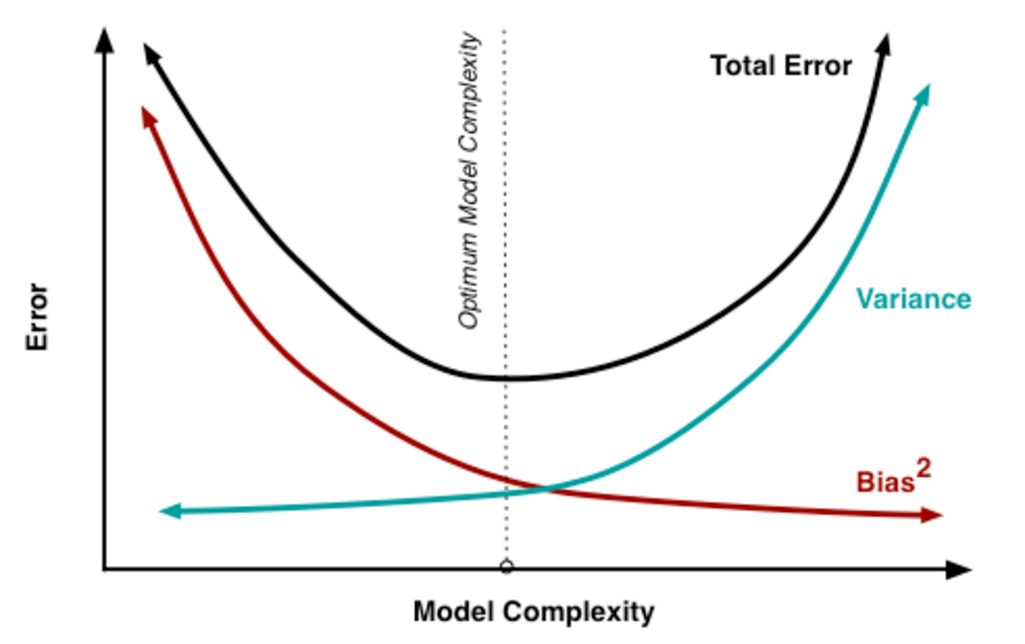
\includegraphics{figures/modelcomplexity.pdf}
      }
    }
    \only<2>{\resizebox{\textwidth}{!}{
        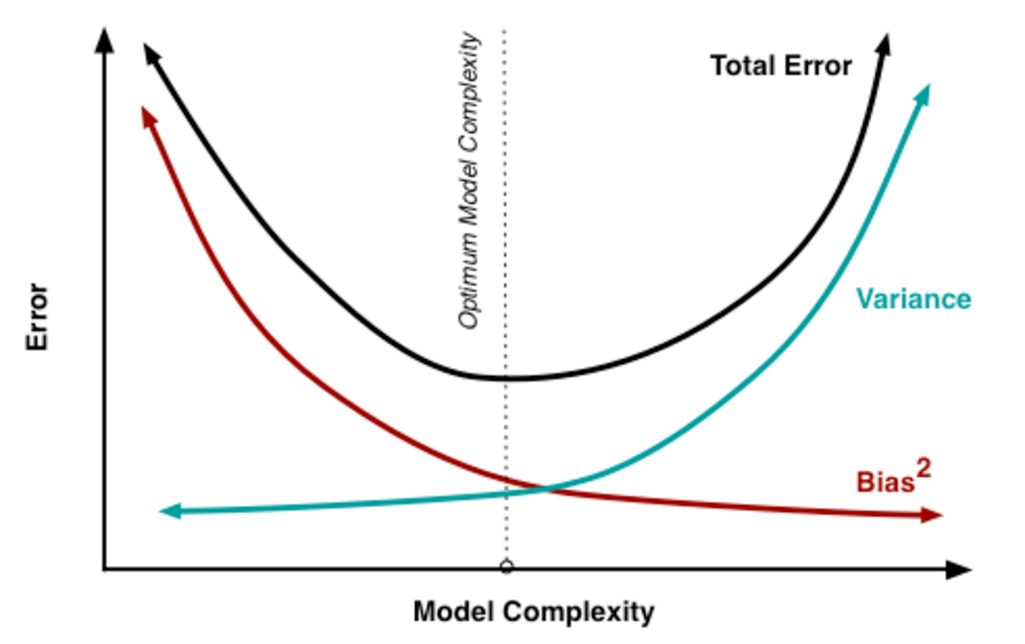
\includegraphics{figures/modelcomplexity.pdf}
      }
    }
    \only<3>{\resizebox{\textwidth}{!}{
        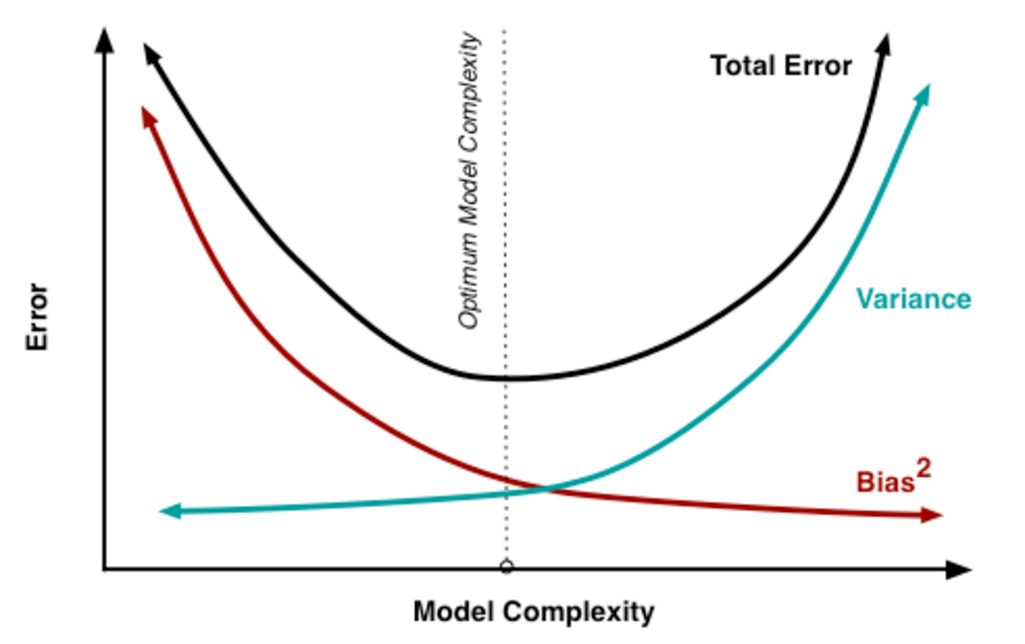
\includegraphics{figures/modelcomplexity.pdf}
      }
    }
  \end{column}
  \hfill
  \begin{column}{.4\textwidth}
    \footnotesize
    \begin{wideitemize}\footnotesize
    \item<1-> Model complexity is across the $x$ axis and model error across
    the $y$ axis. More complexity means higher variance. Lesser complexity
    means higher bias.
    \item<2-> So this what bias/variance tradeoff is all about: \textbf{finding
    the right model complexity} that minimizes both bias and variance (I mean
    the total error as much as possible.
    \item<3-> Total error is very high for very simple models and a very complex
    model, and then it bottoms out in the middle.
    \end{wideitemize}
    \end{column}
  \end{columns}
  % \begin{wideitemize}
  %   \item Model complexity is across the $x$ axis and model error across
  %   the $y$ axis. More complexity means higher variance. Lesser complexity
  %   means higher bias.
  %   \item Total error is very high for very simple models and a very complex
  %   model, and then it bottoms out in the middle. So this what bias/variance
  %   tradeoff is all about: \textbf{finding the right model complexity} that
  %   minimizes both bias and variance (I mean the total error\footnote{Total
  %   error = (Bias + Variance) + Irreducible Error}) as much as possible.
  % \end{wideitemize}
\end{frame}

% \subsection{Overfitting vs Underfitting}
% \begin{transitionsubframe}
%   \begin{center}
%     \Huge \textbf{What is Overfitting and Underfitting?}
%   \end{center}
% \end{transitionsubframe}

\begin{frame}[fragile]{\textbf{Q. What is Underfitting?}}
  Underfitting occurs when an algorithm cannot capture the underlying trend of the data.
  \begin{columns}[T]
  \begin{column}{.58\textwidth}
    \only<1>{\resizebox{\textwidth}{!}{
        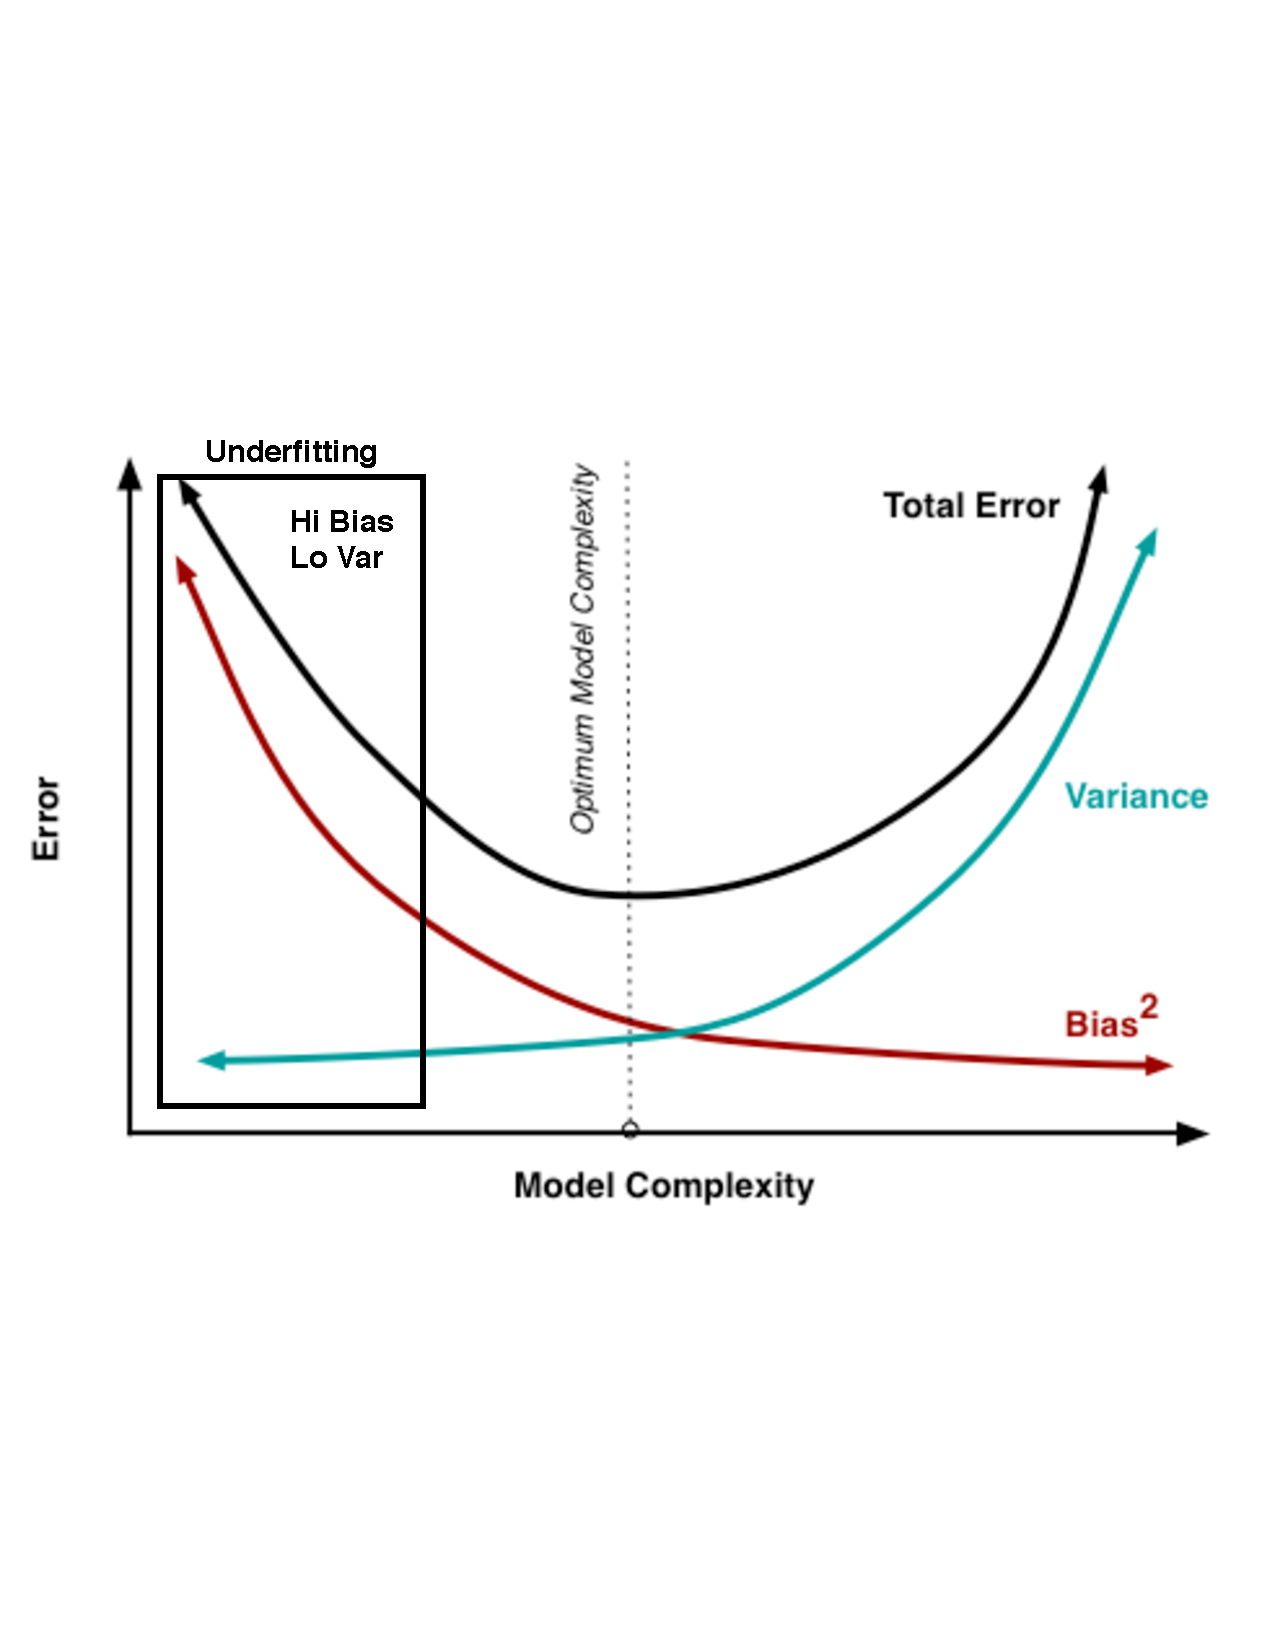
\includegraphics{figures/underfit.pdf}
      }
    }
    \only<2>{\resizebox{\textwidth}{!}{
        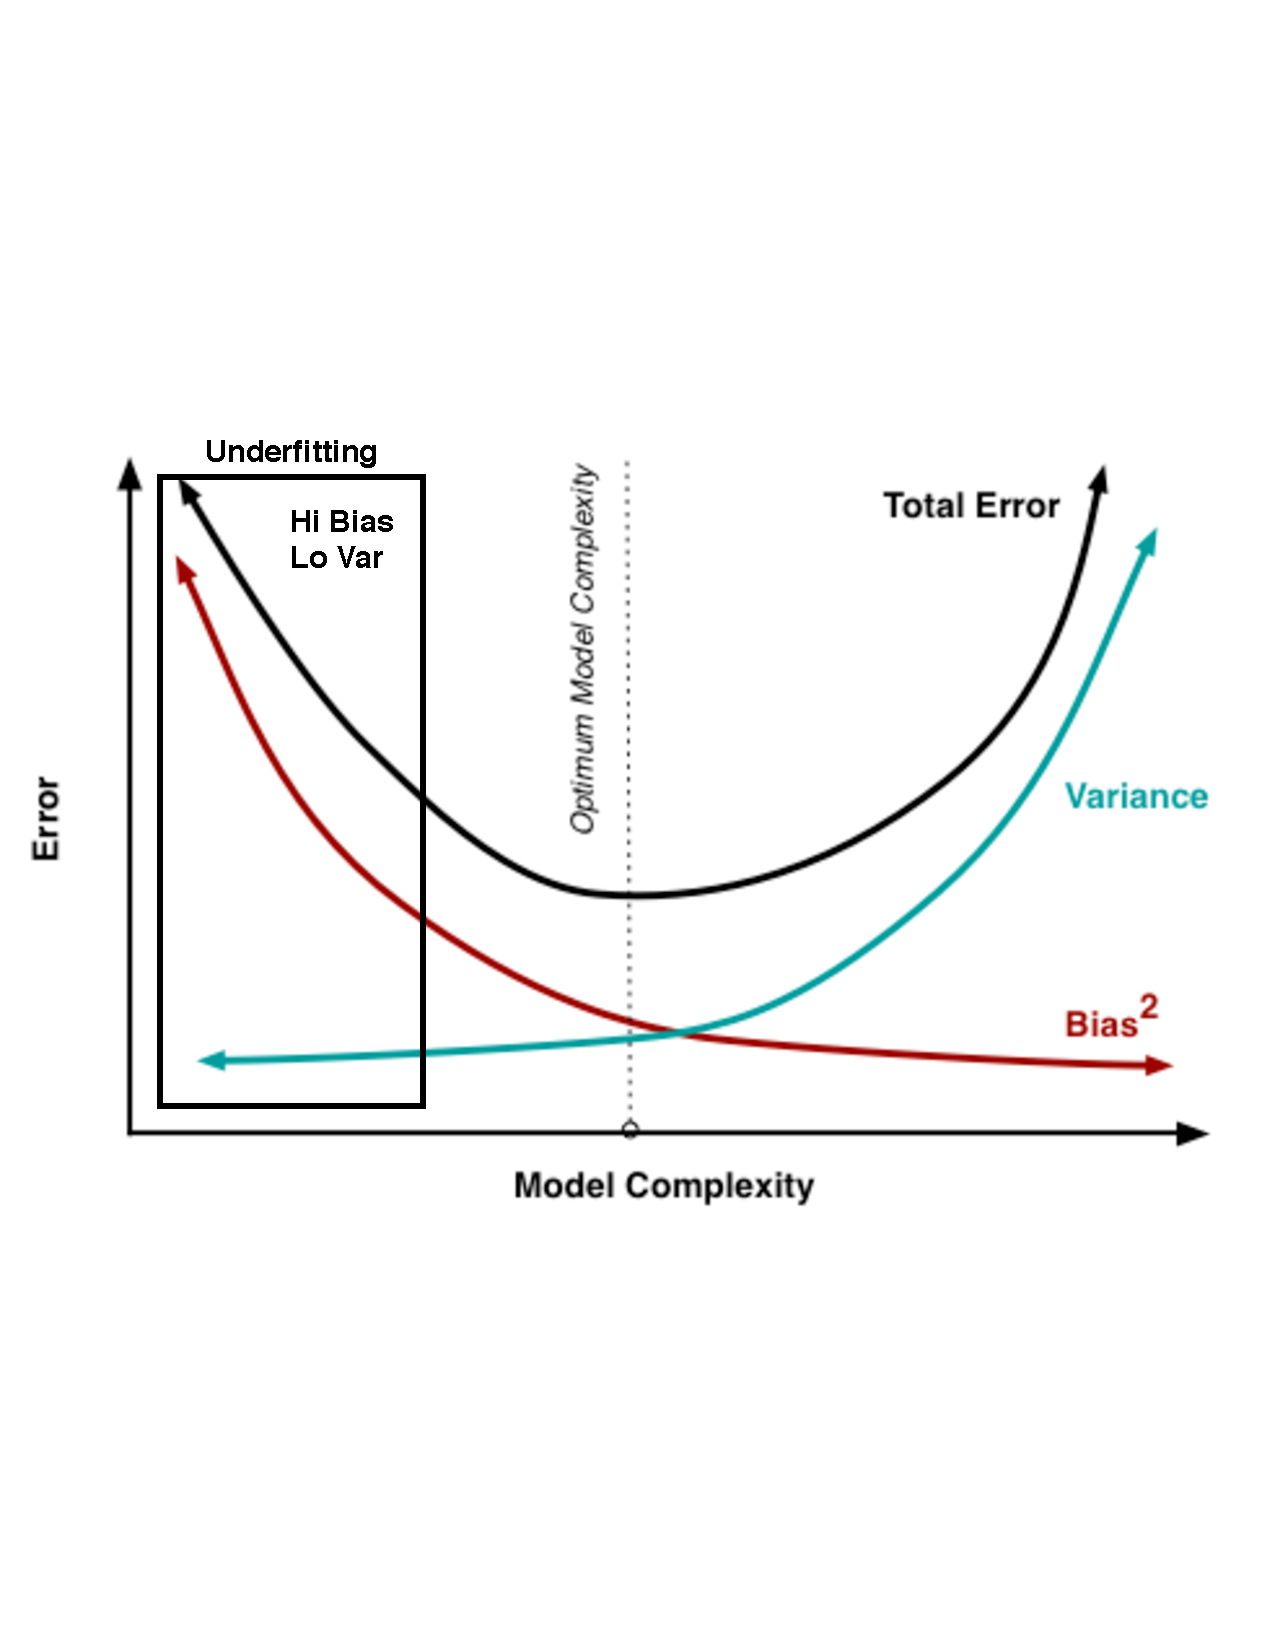
\includegraphics{figures/underfit.pdf}
      }
    }
  \end{column}
  \hfill
  \begin{column}{.4\textwidth}
    \footnotesize
    \begin{wideitemize}
      \item<1-> Underfitting happens when the model is too simple with high bias
      and low variance, and results in high total error.
      \item<2-> \textbf{Underfitting}: High bias + low variance
    \end{wideitemize}
    \end{column}
  \end{columns}
  % \begin{wideitemize}
  %   \item (Recall high bias.) Underfitting occurs when an algorithm
  %   cannot capture the underlying trend of the data. This happens
  %   when the model is too simple with high bias and low variance, and
  %   results in high total error.
  %   \item Underfitting: High bias + low variance (The left side of this plot represents underfitting).
  % \end{wideitemize}
\end{frame}

\begin{frame}[fragile]{\textbf{Q. What is Overfitting?}}
  Overfitting occurs when an algorithm
  fits too closely to a limited set of data (i.e., training set).
  \begin{columns}[T]
  \begin{column}{.58\textwidth}
    \only<1>{\resizebox{\textwidth}{!}{
        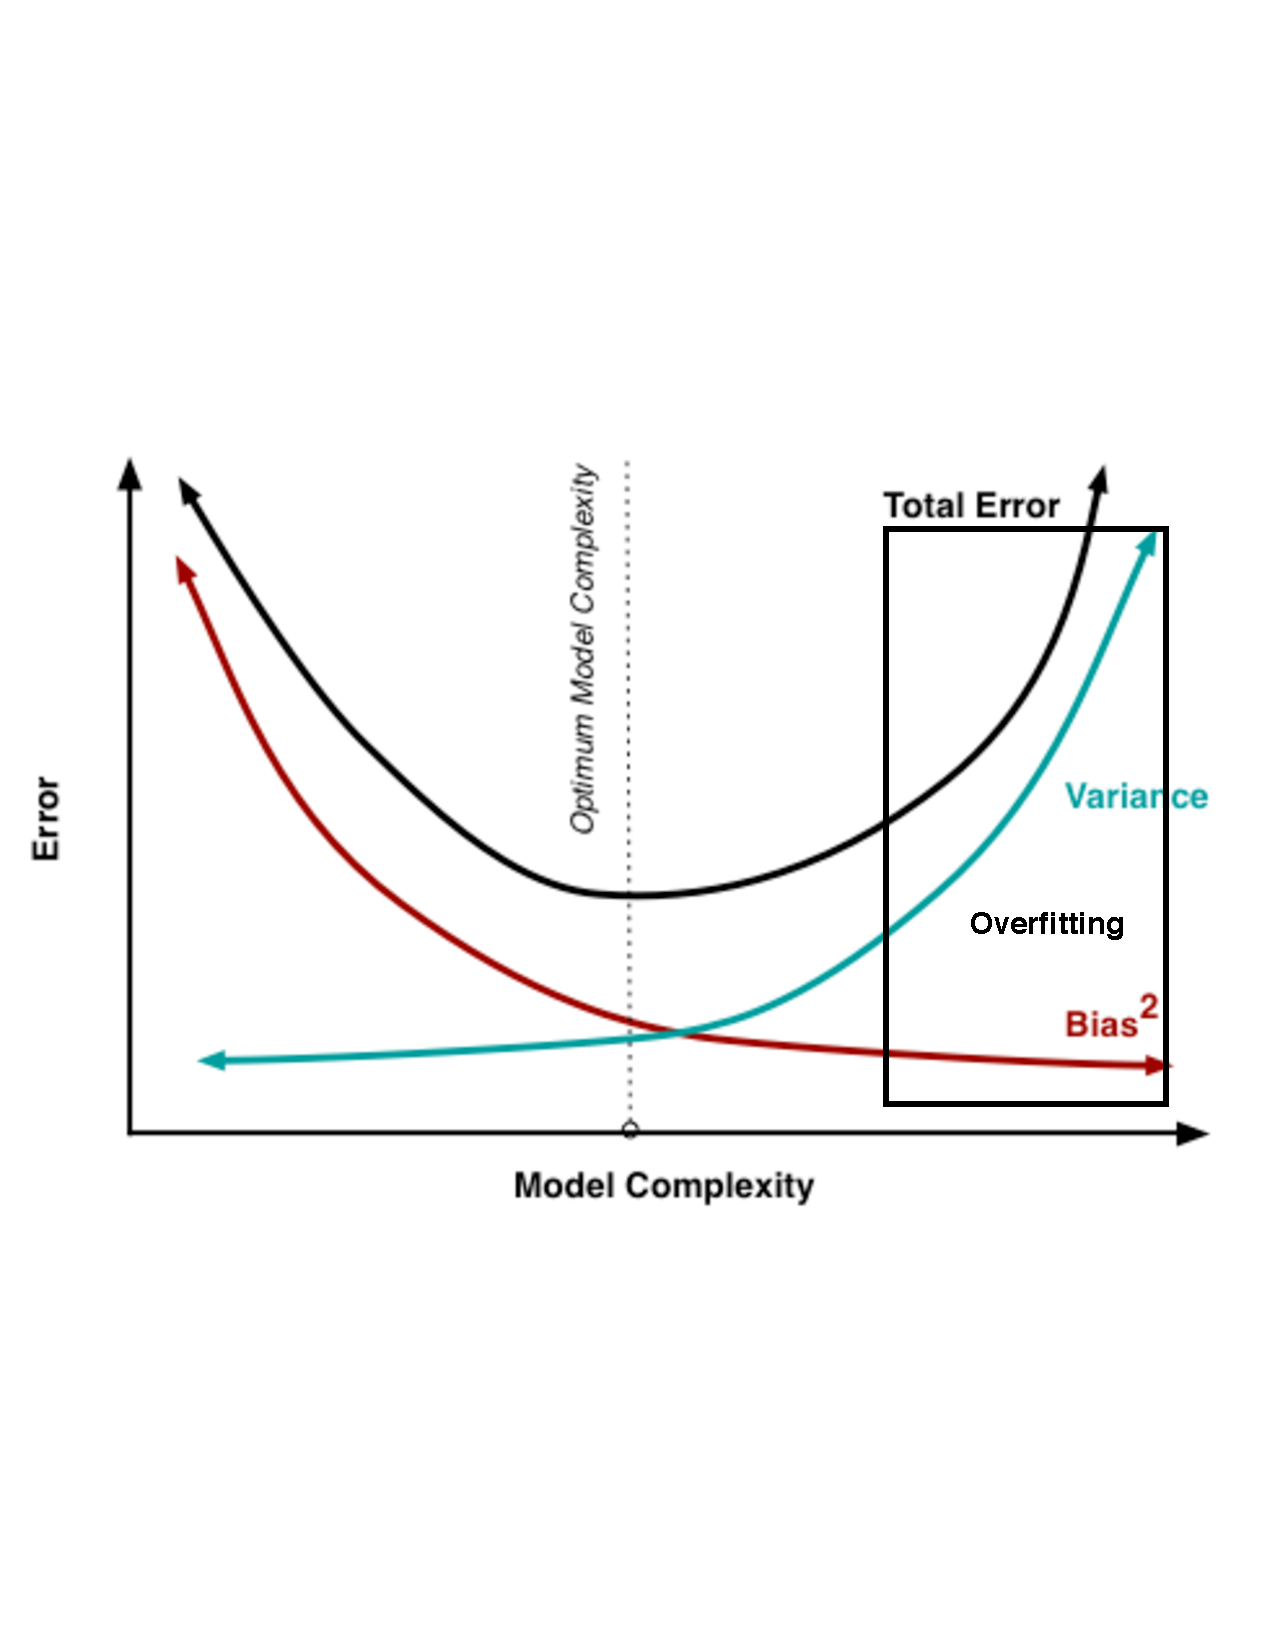
\includegraphics{figures/overfit.pdf}
      }
    }
    \only<2>{\resizebox{\textwidth}{!}{
        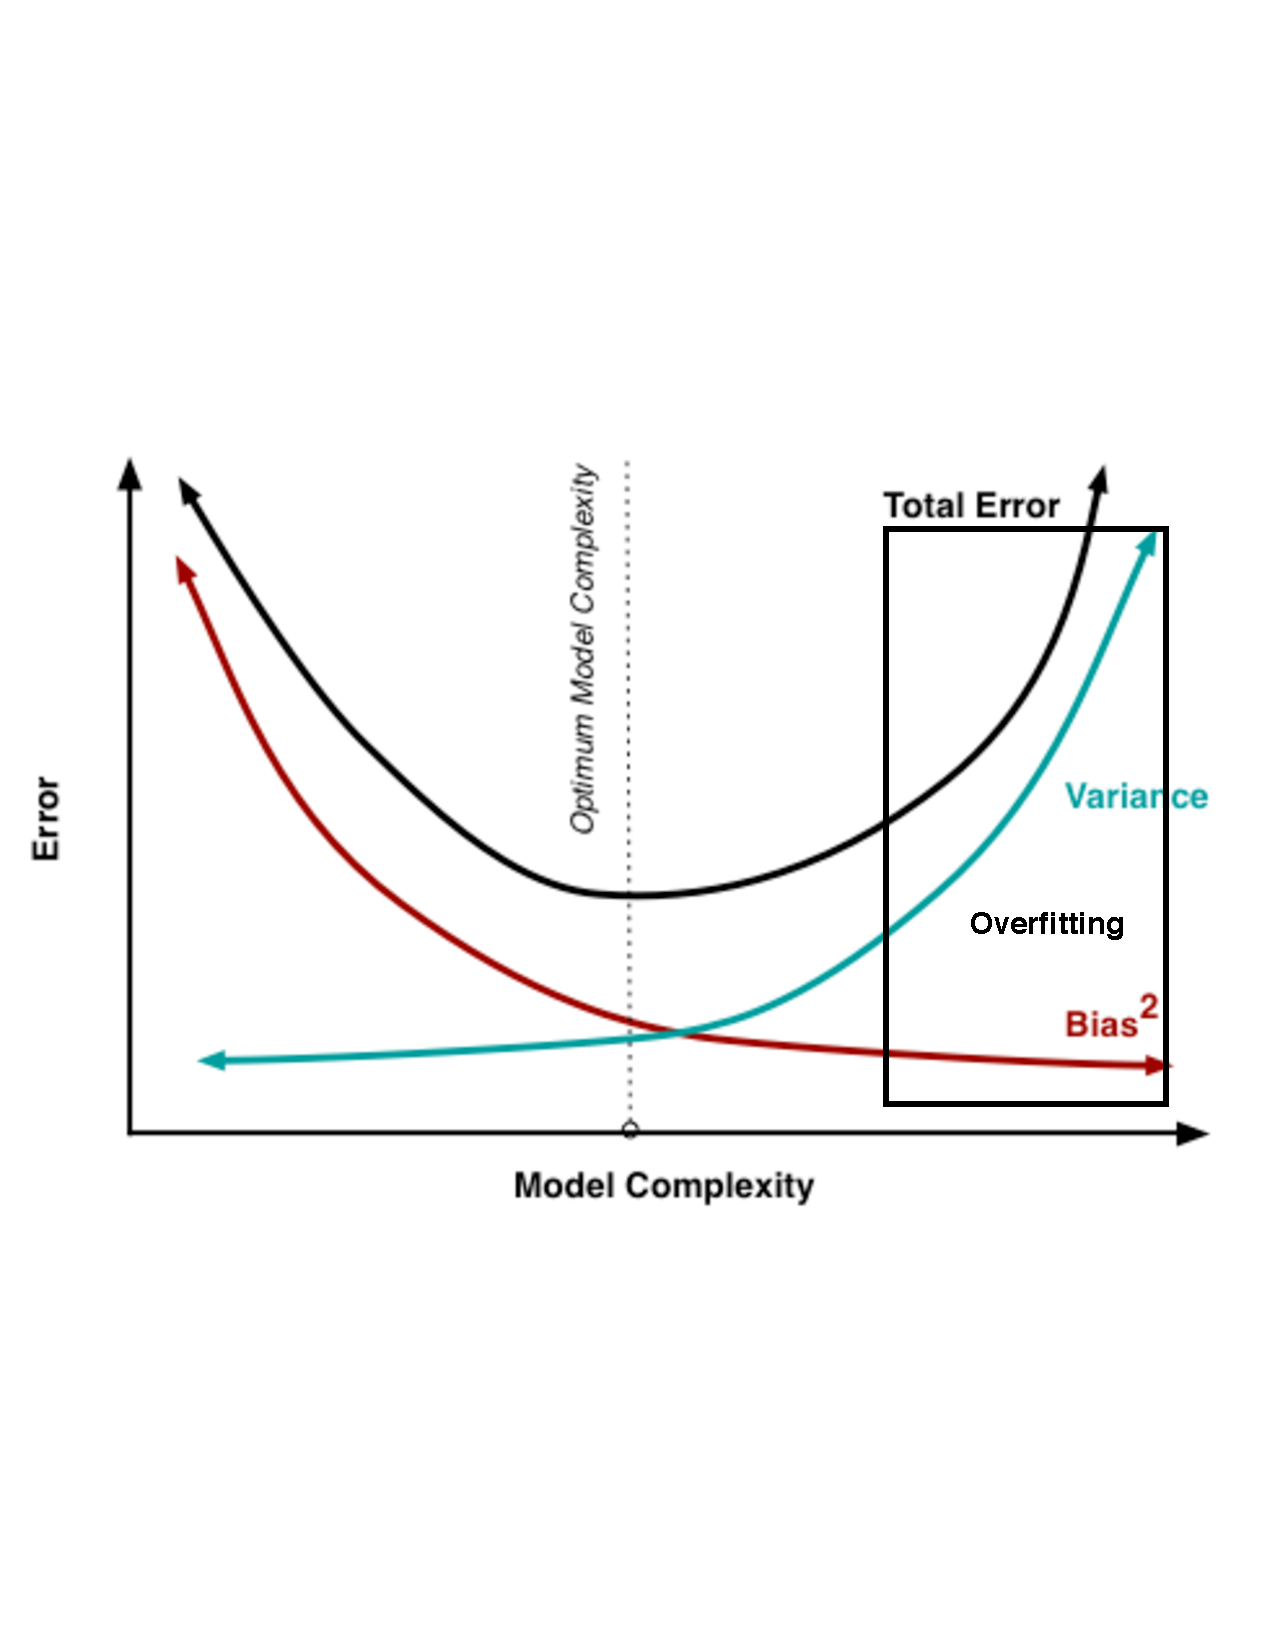
\includegraphics{figures/overfit.pdf}
      }
    }
  \end{column}
  \hfill
  \begin{column}{.4\textwidth}
    \footnotesize
    \begin{wideitemize}
      \item<1-> In other words, the model might just memorize the examples that it has seen in
      the training data.\medskip
      % \begin{wideitemize}
      %   \item<1-> Then when it sees a new example that looks a lot like an
      %   example it has seen before it can make a very accurate prediction.
      %   \item<1-> And when it sees a new example that looks nothing like any
      %   other examples it has seen before it will make a very poor prediction.
      % \end{wideitemize}
      \item<2-> \textbf{Overfitting}: Low bias + high variance.
    \end{wideitemize}
    \end{column}
  \end{columns}

  % \begin{wideitemize}
  %   \item<1-> (Recall high variance.) Overfitting occurs when an algorithm
  %   fits too closely to a limited set of data (i.e., training set). In other
  %   words, the model might just memorize the examples that it has seen in
  %   the training data.\medskip
  %   \begin{wideitemize}
  %     \item<1-> Then when it sees a new example that looks a lot like an
  %     example it has seen before it can make a very accurate prediction.
  %     \item<1-> And when it sees a new example that looks nothing like any
  %     other examples it has seen before it will make a very poor prediction.
  %   \end{wideitemize}
  %   \item<2-> \textbf{Overfitting}: Low bias + high variance.
  % \end{wideitemize}
\end{frame}

\subsection{Finding optimal model complexity}
\begin{transitionsubframe}
  \begin{center}
    \Huge \textbf{The actual process?}
  \end{center}
\end{transitionsubframe}

\begin{frame}[fragile]{\textbf{Q. How do you find the optimal tradeoff?}}
  \begin{wideitemize}
    \item The goal is to find something in the middle\footnote{This would learn the
    true pattern in the data w/o memorizing every example in the training data.} (a
    model with medium complexity); i.e., \textbf{Optimal tradeoff:} Low bias + Low variance.
    \item OKAY, \textcolor{red}{but how do you identify underfit and overfit?}
    % \begin{wideitemize}
    %   \item With underfit, we'll have high training error and high test error.
    %   \item Optimal tradeoff, we'll have low training error and low test error.
    %   \item With overfit, we'll have low training error and high test error.
    % \end{wideitemize}
  \end{wideitemize}

  \begin{columns}[T]
  \begin{column}{.58\textwidth}
    \only<1>{\resizebox{\textwidth}{!}{
        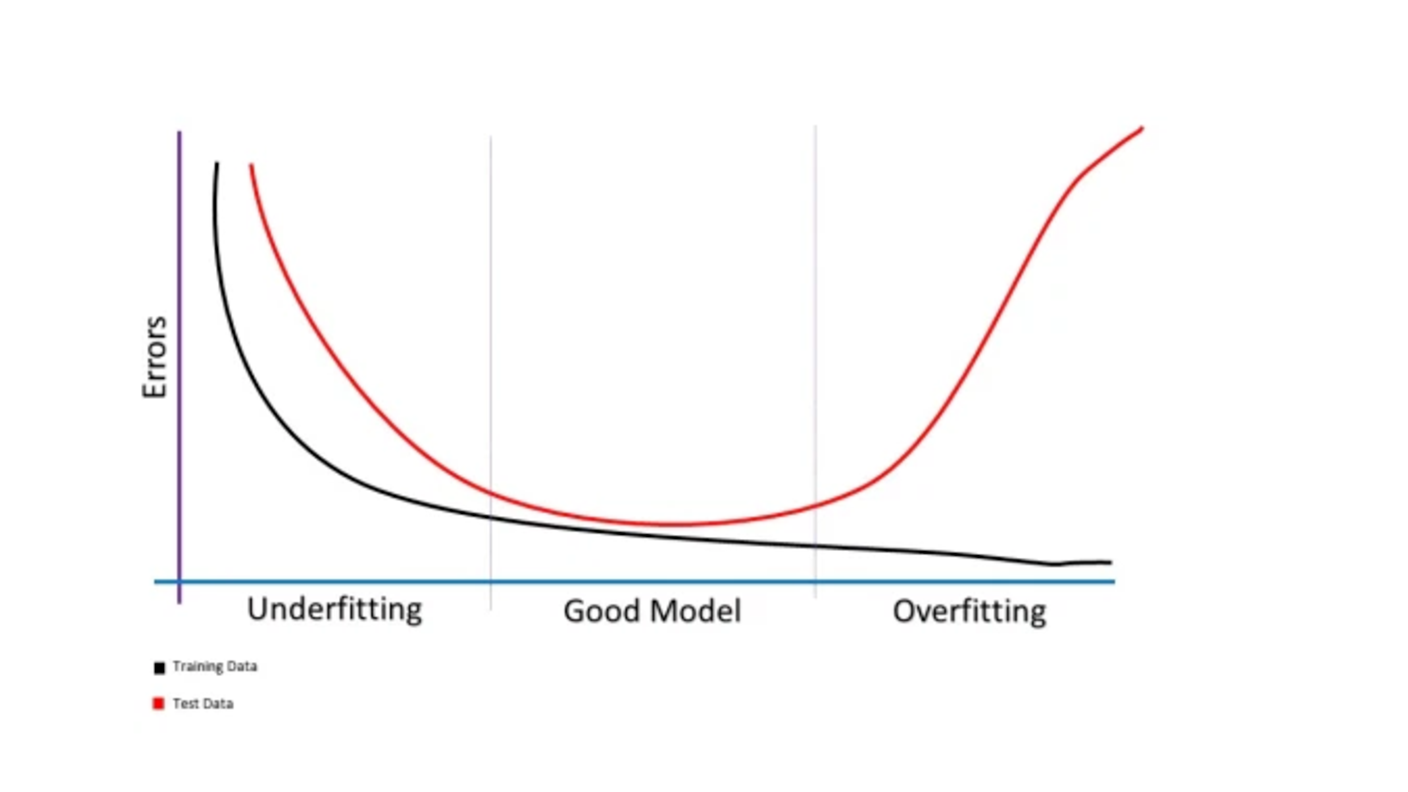
\includegraphics{figures/detectunderandoverfit.pdf}
      }
    }
    \only<2>{\resizebox{\textwidth}{!}{
        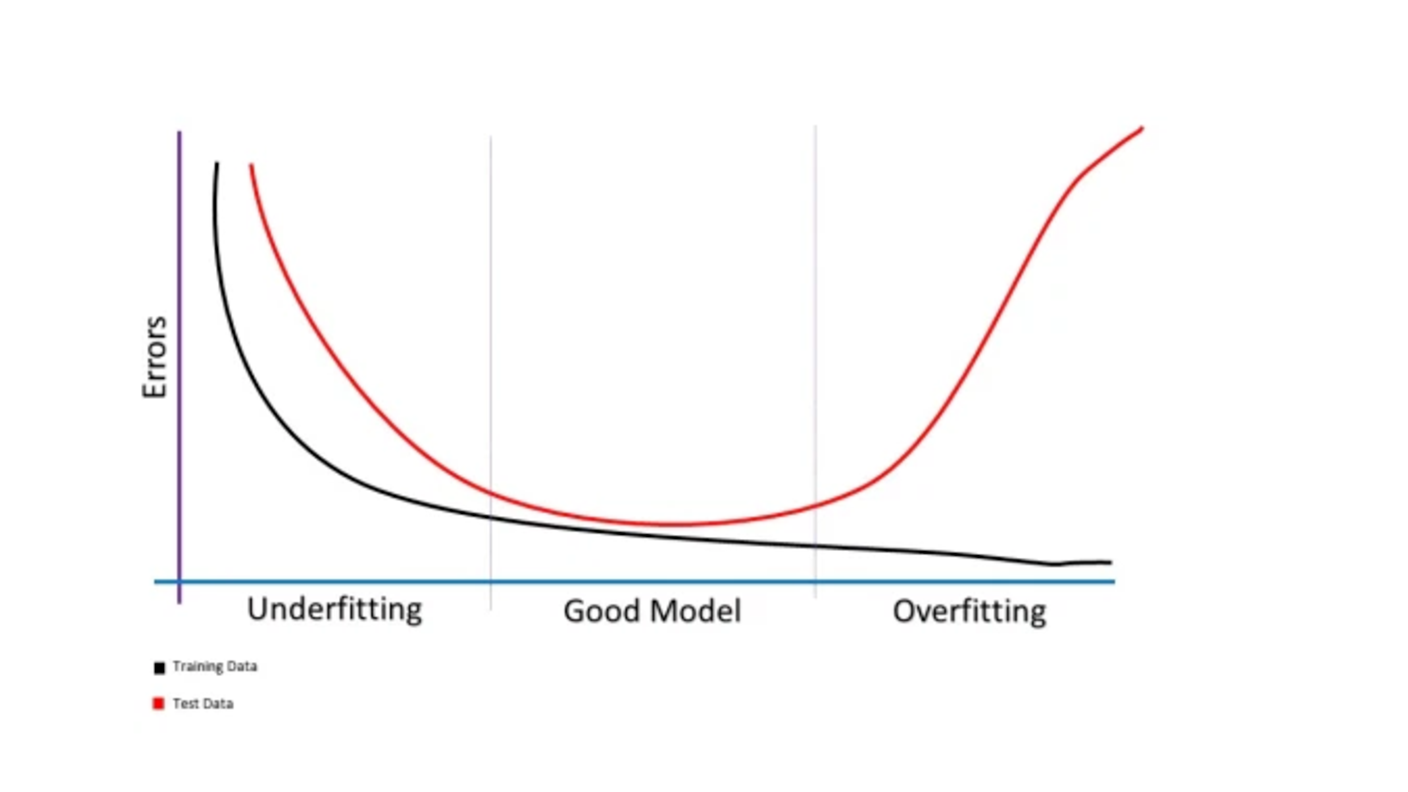
\includegraphics{figures/detectunderandoverfit.pdf}
      }
    }
    \only<3>{\resizebox{\textwidth}{!}{
        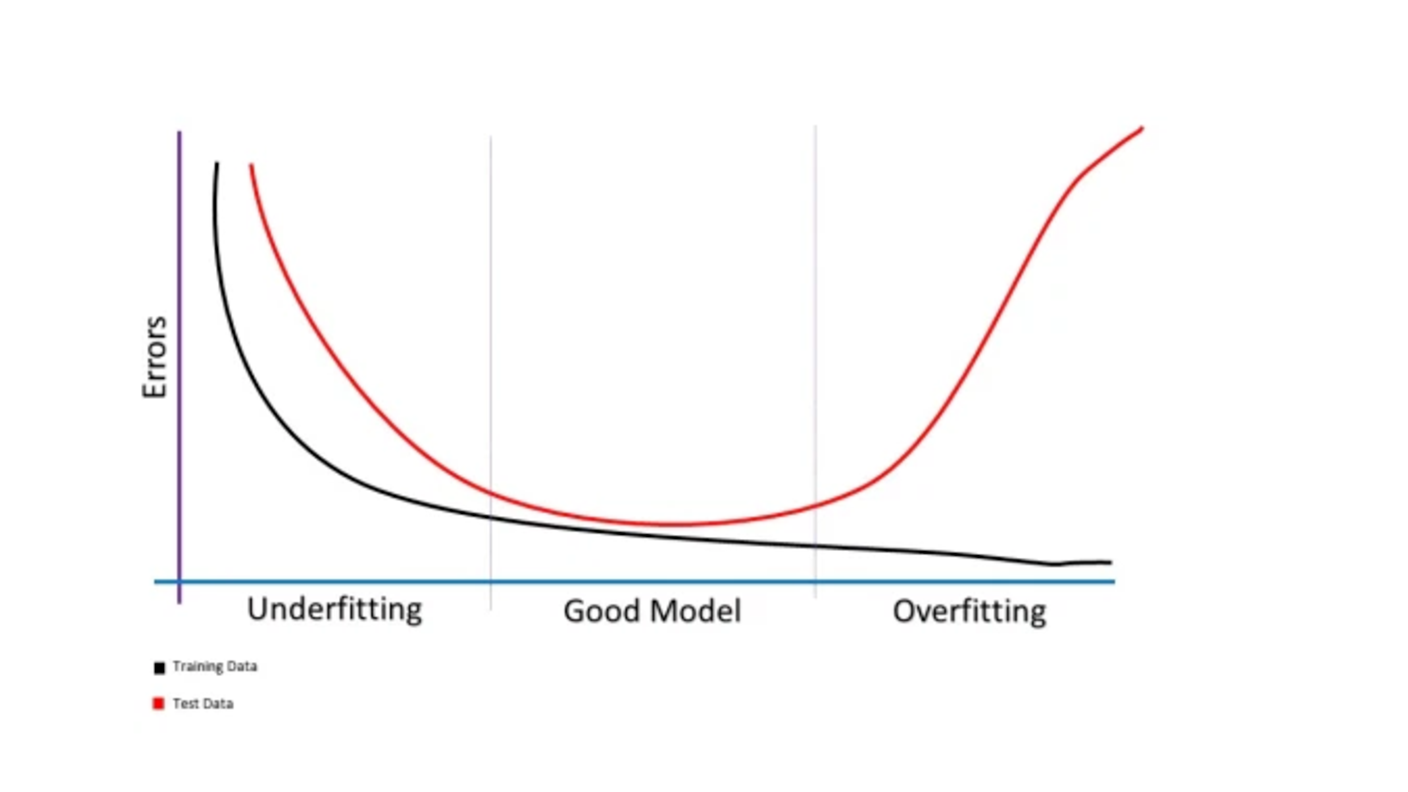
\includegraphics{figures/detectunderandoverfit.pdf}
      }
    }
  \end{column}
  \hfill
  \begin{column}{.4\textwidth}
    \footnotesize
    \begin{wideitemize}\footnotesize
    \item<1-> With underfit, we'll have high training error and high test error.
    \item<2-> Optimal tradeoff, we'll have low training error and low test error.
    \item<3-> With overfit, we'll have low training error and high test error.
    \end{wideitemize}
    \end{column}
  \end{columns}
\end{frame}

\note[itemize]{
\item The goal is to find something in the middle (a model with medium
complexity). This would learn the true pattern in the data w/o memorizing
every example in the training data.
}

\begin{frame}[fragile]{\textbf{Q. How do you tune a model for optimal complexity?}}
  \begin{wideitemize}
    \item There are two methods to tune a model for optimal complexity:\medskip
    \begin{wideitemize}
      \item Hyper-parameter tuning -- choosing a set of optimal hyper-parameters
      for fitting a ML algorithm (e.g., linear regression)
      \item Regularization -- a technique used specifically to reduce overfitting
      by discouraging overly complex models in some way.
    \end{wideitemize}
  \end{wideitemize}
\end{frame}

\begin{frame}[fragile]{\textbf{Q. What is a hyper-parameter?}}
  \begin{wideitemize}
    \item A model \textbf{parameter} is a configuration variable that
    is internal to the model and \textit{whose value can be estimated from data}.
    \item A model \textbf{hyper-parameter} is a configuration that is external
    to the model and \textit{whose value cannot estimated from data}, and
    \textit{whose value guides how the algorithm learns parameter values from
    the data}. E.g., depth of a decision tree is a model hyper-parameter vs
    ticket price or ticket class are model parameters.
  \end{wideitemize}
\end{frame}

\begin{frame}[fragile]{\textbf{Q. What is Regularization?}}
  \begin{wideitemize}
    \item Regularization is a form of regression, which constrains/regularizes or shrinks
    the (learned) coefficient estimates towards zero. In other words, this technique
    reduces overfitting by discouraging learning a more complex model in some way.
  \end{wideitemize}
  \begin{framed}
    The goal of Regularization is to allow enough flexibility for the algorithm
    to learn the underlying patterns in the data but provides guardrails so it
    doesn't overfit. See Occam's razor -- whenever possible, choose the simplest
    model to a problem.
  \end{framed}
\end{frame}

\begin{frame}[fragile]{\textbf{Q. Can you provide Regularization examples?}}
  \begin{wideitemize}
    \item \textbf{Ridge regression and lasso regression}: adding a penalty
    to the loss function (See Model fitting slide) to constrain coefficients.
    \item \textbf{Dropout}: some nodes are ignored during training which
    forces the other nodes to take on more or less responsibility for the
    input-output.
  \end{wideitemize}
\end{frame}

\subsection{Unpacking terms}
\begin{transitionsubframe}
  \begin{center}
    \Huge Epoch vs Batch size vs Iteration
  \end{center}
\end{transitionsubframe}

\begin{frame}[fragile]{\textbf{Q. What is the difference between these terms?}}
  \begin{wideitemize}
    \item To find out the difference between these terms you need to know some
    of the machine learning terms like Gradient Descent to help you better
    understand.
  \end{wideitemize}
\end{frame}


\begin{frame}[fragile]{\textbf{Q. What is Gradient Descent?}}
  \begin{wideitemize}
    \item Gradient descent is an \textit{iterative} optimization algorithm used to minimize
    some \textit{convex} function by \textit{iteratively} moving in the direction of
    steepest descent as defined by the negative of the gradient.
    \item In ML, we use gradient descent to update the parameters of a ML model.\medskip
    \begin{wideitemize}
      \item Start with an initial guess for each parameter $\theta_{k}$. Then
      move $\theta_{k}$ in the \\direction of the slope.
      \item Update all $\theta_{k}$ parameters simultaneously (known as batch gradient descent),
      and \\repeat until convergence.
    \end{wideitemize}
  \end{wideitemize}
\end{frame}

\begin{frame}[fragile]{\textbf{Q. Unpacking Gradient Descent?}}
  \begin{wideitemize}
    \item Gradient means the rate of inclination or declination of a slope.
    \item Descent means we are dealing with the inclination of a slope.
    \item The algorithm is iterative means that we need to get the results
    \textbf{multiple times} to get the most optimal result (minima of a curve).
  \end{wideitemize}
\end{frame}

\begin{frame}[fragile]{\textbf{Q. What is Stochastic Gradient Descent?}}
  \begin{wideitemize}
    \item Similar to batch gradient descent except that you only update
    using one of the data points each time.
    \item And that data point is chosen randomly. Hence the stochastic.
    \item In other words, stochastic gradient descent pick an $n$ at random
    and then update using one of the data points. Repeat, picking another
    data point at random, etc.
  \end{wideitemize}
\end{frame}

\begin{frame}[fragile]{\textbf{Q. What is an epoch?}}
  \begin{wideitemize}
    \item In some ML methods, one uses the same training data many times,
    as the algorithm gradually converges, for example, in stochastic gradient
    descent. Each time the whole training set of data is used in the training
    that is called an \textbf{epoch}\footnote{Typically you won't
    get decent results until convergence after many epochs}.
    \item One might see a decreasing error as the number of epochs increases.
    But that doesn't mean your algorithm is getting better, it could easily
    mean that you are overfitting\footnote{This could happen if the learning
    algorithm has seen the training data so many times or epochs}. To test for
    this you introduce a test data set, the data that you've held back.
  \end{wideitemize}
\end{frame}

\begin{frame}[fragile]{\textbf{Q. So, what is the right numbers of epochs?}}
  \begin{wideitemize}
    \item Unfortunately, there is no right answer to this question. The answer
    is different for different data sets but you can say that the numbers of
    epochs is related to how diverse your data is. For example, do you have
    only black cats in your data set or is it much more diverse dataset?
  \end{wideitemize}
\end{frame}

\begin{frame}[fragile]{\textbf{Q. What is a batch?}}
  \begin{wideitemize}
    \item As I said, you can't pass the entire data set into a ML algorithm at
    once. So, you divide data set into a number of batches or sets or parts.
  \end{wideitemize}
\end{frame}

\begin{frame}[fragile]{\textbf{Q. What is an iteration?}}
  \begin{wideitemize}
    \item An iteration is the number of batches needed to complete one epoch.
    \item Let's say we have 2000 training examples that we are going to use.
    \begin{wideitemize}
      \item We can divide the dataset of 2000 examples into batches of 500
      then it will take 4 iterations to complete 1 epoch.
    \end{wideitemize}
  \end{wideitemize}
\end{frame}

\section{End-to-End Pipeline}
\begin{transitionframe}
  \begin{center}
    \Huge End-to-End Pipeline\\(starting from fit initial model)
  \end{center}
\end{transitionframe}

\subsection{Fitting a basic model}
\begin{transitionsubframe}
  \begin{center}
    \Huge Run fivefold cross-validation and select the best models.
  \end{center}
\end{transitionsubframe}

\begin{frame}[fragile]{\textbf{Q. Fit a basic model using cross validation?}}
  \begin{wideitemize}
    \item Goal: To understand what the baseline performance looks like
    \footnote{We'll use only the training set}.
    \begin{wideitemize}
      \item From sklearn, import RandomForestClassifier, and cross-val-score
      to compute the accuracy of the baseline model.
    \end{wideitemize}
    \item Next, we will select other models in order to beat our baseline.
  \end{wideitemize}
\end{frame}

\begin{frame}[fragile]{\textbf{Q. Tunning Hyper-parameters?}}
  \begin{wideitemize}
    \item Run grid search to find the optimal hyper-parameter settings for our models.
    \item Our goal of this step is to find the optimal model that beats that baseline performance.
    \item We use GridSearchCV\footnote{a wrapper around cross fail score that allows us to
    run grid search within cross validation.}, which yields multiple combinations of hyper-params
    values, to find the combinations that improves performance\footnote{Recall that a model is a
    configuration of the ML algorithm on specific params values}.
    % \begin{wideitemize}
    %   \item Go ahead and import this random forest classifier again, but now
    %   instead of using cross fail score, we will use \textit{GridSearchCV}, and
    %   all GridSearchCV is, is a wrapper around cross fail score, that allows us to
    %   run grid search within cross validation.
    %   \item GridSearchCV yields multiple combinations of hyper-params values and finds the
    %   combinations that improves performance\footnote{Recall that a model is a configuration
    %   of the ML algorithm on specific params values}.
    % \end{wideitemize}
  \end{wideitemize}
\end{frame}

\subsection{Re-fit models on full training set}
\begin{transitionsubframe}
  \begin{center}
    \Huge Re-fit models on full training set, evaluate those models
    on the validation set and pick the best one.
  \end{center}
\end{transitionsubframe}

\begin{frame}{\textbf{Q. Evaluating results on Validation set?}}
  \begin{wideitemize}\small
    \item Now that we've done some hyper parameter tuning, and we have a good idea
    of what the best hyper parameter combinations are, let's evaluate these models on
    the validation set\footnote{Now the performance shouldn't deviate too much from
    the performance we saw with the cross-validation.}.
    \item The process goes like this:
    \begin{wideitemize}
      \item[1] Look at additional performance metrics beyond just accuracy
      (e.g., precision and recall) and also at different ML algorithms.
      \item[2] Take the $3$ best performing models and \textbf{re-fit} them
      using the whole training data\footnote{Why do we need to do that? Because
      these models were fit on only $80$\% of the training data; we need now the entire training data.}.
      \item[3] Evaluate these models on the validation set\footnote{This is the truth test.
      If they are overfit or underfit, then they will fail here.}.
      \item[4] Select the best performing model.
    \end{wideitemize}
  \end{wideitemize}
\end{frame}

\subsection{Evaluate that best model}
\begin{transitionsubframe}
  \begin{center}
    \Huge Evaluate that best model on the test set to gauge its ability
    to generalize to unseen data.
  \end{center}
\end{transitionsubframe}

\begin{frame}[fragile]{\textbf{Q. Final model selection and evaluation on test set?}}
  \begin{wideitemize}\small
    \item Next, we'll evaluate the best model on the test set. This will give us
    a truly unbiased view of how it should preform moving forward.
    \item Why do we need to evaluate it on test data, given they have already evaluated on unseen data?
    \medskip
    \begin{wideitemize}
      \item For the validation set was created by \textbf{randomly} distributing examples from
      the full data set. So if that validation set was slightly different perhaps we would
      have chosen a different model.
      \item So by nature of this fact that testing on the validation set impacted what model
      was chosen as our final model, it's technically part of the model training process.
      \item So this final test set is purely for evaluation purposes to see that it matches
      the performance that we've seen before and to give us more confidence in the performance
      of the model moving forward.
    \end{wideitemize}
  \end{wideitemize}
\end{frame}

\section{Algorithms}
\begin{transitionframe}
  \begin{center}
    \Huge Machine Learning Algorithms
  \end{center}
\end{transitionframe}

\subsection{Regression}
\begin{transitionsubframe}
  \begin{center}
    \Huge Regression algorithms (Supervised learning)
  \end{center}
\end{transitionsubframe}

\begin{frame}[fragile]{\textbf{Q. What is Regression?}}
  \begin{wideitemize}
  \item \textbf{Regression} is a statistical process for estimating
  the relationship among variables, often used to make a prediction about
  some outcome.\medskip
  \begin{wideitemize} 
    \item \textit{From a Machine Learning perspective, the modeling of this relationship
    is done to ensure generalization -- giving the model the ability to predict
    outputs (dependent variable) for inputs (independent variables) it has never
    seen before.}
  \end{wideitemize}
  \end{wideitemize}
\end{frame}


\begin{frame}[fragile]{\textbf{Q. What is linear regression?}}
  \begin{wideitemize}
  \item \textbf{Linear regression} is one type of regression that is used when
  trying to predict a continuous target variable (output).\medskip
  \begin{wideitemize}
    \item The essence of LR is that given some correlated data, LR tries to
      explain a dependent variable in terms of independent variables.
    \item The independent variables are numerical (continuous) and we \textit{fit} straight
      lines, polynomials or other functions to predict the dependent variables.
  \end{wideitemize}
  \item Example: Find a relationship between the number of tomatoes on a plant
    and how much they are watered. Using the algorithm definition for linear
    regression is $y = mx + b$, where $y$ is the tomatoes number (dependent
    var), $x$ is how much they are watered (independent var), and $b$ and $m$
    (i.e., slope) are coefficients dictating the best fit line\footnote{e.g., a
      model that assumes a linear relationship between the input}.
    {\footnotesize Based on the water data, you could infer the number of tomatoes on a
      plant for an amount of water for which we don't any data.}\medskip
  % \item Linear regression attempts to model the relationship between two continuous
  %   variables -- a scalar response (or dependent variable) and and one or more
  %   explanatory variables (or independent variables) -- by fitting a linear
  %   equation to observed data.
  % \item The governing algorithm or equation for linear regression is also quite simple.
  %   It takes the form: $y = mx + b$ where $y$ is the dependent variable, $x$ is the
  %   independent variable, and $b$ and $m$ (i.e., slope) are coefficients
  %   dictating the equation.
  % \item e.g. a model that assumes a linear relationship between the input
  %   variables $x$ and the single output variable $y$.
  \end{wideitemize}
\end{frame}

\begin{frame}[fragile]{\textbf{Q. How does linear regression work?}}
  \begin{wideitemize}
  \item The way Linear Regression works is by trying to find the weights (namely, $m$ and $b$)
  that lead to the best-fitting line for the input data (i.e. X features) we have.
  The best-fitting line is determined in terms of \textbf{lowest cost}.\medskip
  \begin{wideitemize}
    \item Generally, cost refers to the loss or error that the model yields in terms
    of \textit{how off it is from the actual Training data}.
    \item When it comes to Linear Regression, the \textbf{cost function} we usually
    use is the Squared Error Cost (i.e., Mean Square Error):
    $\frac{1}{N} \sum_{i=1}^N (y_{i}-(mx_{i} + b))^2$
    \item Using Gradient descent, it tries to find the values for $m$ and $b$
      that will give you the lowest MSE score. (Training is basically finding
      these values.) \textbf{The best fitted line is the one with the lowest MSE value.}
  \end{wideitemize}
  % \item Linear regression attempts to model the relationship between two continuous
  %   variables -- a scalar response (or dependent variable) and and one or more
  %   explanatory variables (or independent variables) -- by fitting a linear
  %   equation to observed data.
  % \item The governing algorithm or equation for linear regression is also quite simple.
  %   It takes the form: $y = mx + b$ where $y$ is the dependent variable, $x$ is the
  %   independent variable, and $b$ and $m$ (i.e., slope) are coefficients
  %   dictating the equation.
  % \item e.g. a model that assumes a linear relationship between the input
  %   variables $x$ and the single output variable $y$.
  \end{wideitemize}
\end{frame}



\begin{frame}[fragile]{\textbf{Q. Linear regression on many dimensions?}}
  \begin{wideitemize}
    \item We now have $M$ independent, explanatory, variables, representing the
      features, and we write all $x_s$ as vectors. For each of $N$ data points
      we'll have the independent variable $x^{(n)}$ (e.g., squared footage of a
      house, number of rage bays) and the independent variable $y^{(n)}$
      (property value).
    \item We fit the linear function $h_{\theta}(x) = \theta^{T}x$ to the $y_s$,
      where $\theta$ is the vector of the as-yet-unknown parameters.
    \item The cost function remains the same as in the one dimension LR: the
      quadratic function. And the coefficients are learned using batch or
      stochastic gradient descent.
  \end{wideitemize}
\end{frame}


\begin{frame}[fragile]{\textbf{Q. Linear regression Recap?}}
  \begin{wideitemize}
    \item Linear Regression is the process of finding a line that best fits the data
    points available on the plot, so that we can use it to predict output values for
    inputs that are not present in the data.
    \item Performance (and error rates) depends on various factors including the
    how clean and consistent the data is.
    \item In case of bad model performance, we usually go for a \textbf{higher polynomial function}.
    This is basically the introduction of new variables into the Regressor function so
    that we allow more flexibility to it\footnote{However, this will cause the LR line
    not to be a straight line anymore.}
  \end{wideitemize}
\end{frame}

\begin{frame}[fragile]{\textbf{Q. What is logistic regression?}}
  \begin{wideitemize}
  \item \textbf{Logistic regression} or logistic classifier is a form or
    regression where the target variable is binary (zero or one, or true or
    false). It takes the form: $\frac{1}{1 + e^{-(mx + b)}}$
  \item \textbf{Example:} Let's say you wanted to examine the relationship between
    your basketball shooting accuracy and the distance that you shoot from. More
    specifically, you want a model that takes in ``distance from the basket'' in
    feet and spits out the probability that you'll make the shot ($1$ for a make, $0$ for a miss).
  \begin{wideitemize}\vspace{2mm}\small
    \item In this example, the equation $-(mx + b)$, labeled as $z$, represents
    \textit{log(odds of making shot)}\footnote{odss = P(Event) / [1-P(Event)]},
    so the probability of making a shot (i.e., $y$) is $\frac{1}{1 + e^{-z}}$.
    Here, $m$ and $b$ are the coefficients we're interested in finding thru optimization,
    and $x$ is \textit{distance from basket}.
  \end{wideitemize}
  \end{wideitemize}
\end{frame}


\begin{frame}[fragile]{\textbf{Q. Logistic regression example?}}
  \begin{wideitemize}
  \item \textbf{Shooting Baskets}. Generally, the further you get from the basket,
    the less accurately you shoot: when given a small distance, the model should
    predict a high probability and when given a large distance it should predict
    a low probability.
    \begin{wideitemize}\vspace{2mm}\small
    \item In logistic regression the output $Y$ is in log odds. Let's say you shot
      $100$ free throws and made $70$. Based on this sample, your probability of
      making a free throw is $70$\%. Your odds of making a free throw is $2.33$,
      which we want to bound between $0$ and $1$ using \textit{log} and the
      \textit{sigmoid} function as odds go from $0$ to $INF$\footnote{log odds
        are just probability stated another way}:
    \item We can write our logistic regression equation: $z = log(mx + b)$,
      where $m$ and $b$ are the coefficients to be learned.
    \item And to get probability from $z$, which is in log odds, we apply the
      sigmoid function: $\frac{1}{1 + e^{-z}}$\footnote{This shows how we can go
        from a linear estimate of log odds to a probability.} In this case, a
      high probability means you'll be able to shoot and a lot probability means you won't.
  \end{wideitemize}
  \end{wideitemize}
\end{frame}

\begin{frame}[fragile]{\textbf{Q. Why won't Linear Regression work for binary target variables?}}
  In other words, why do we need two regression algorithms?
  \begin{columns}[T]
  \begin{column}{.58\textwidth}
    \only<1>{\resizebox{\textwidth}{!}{
        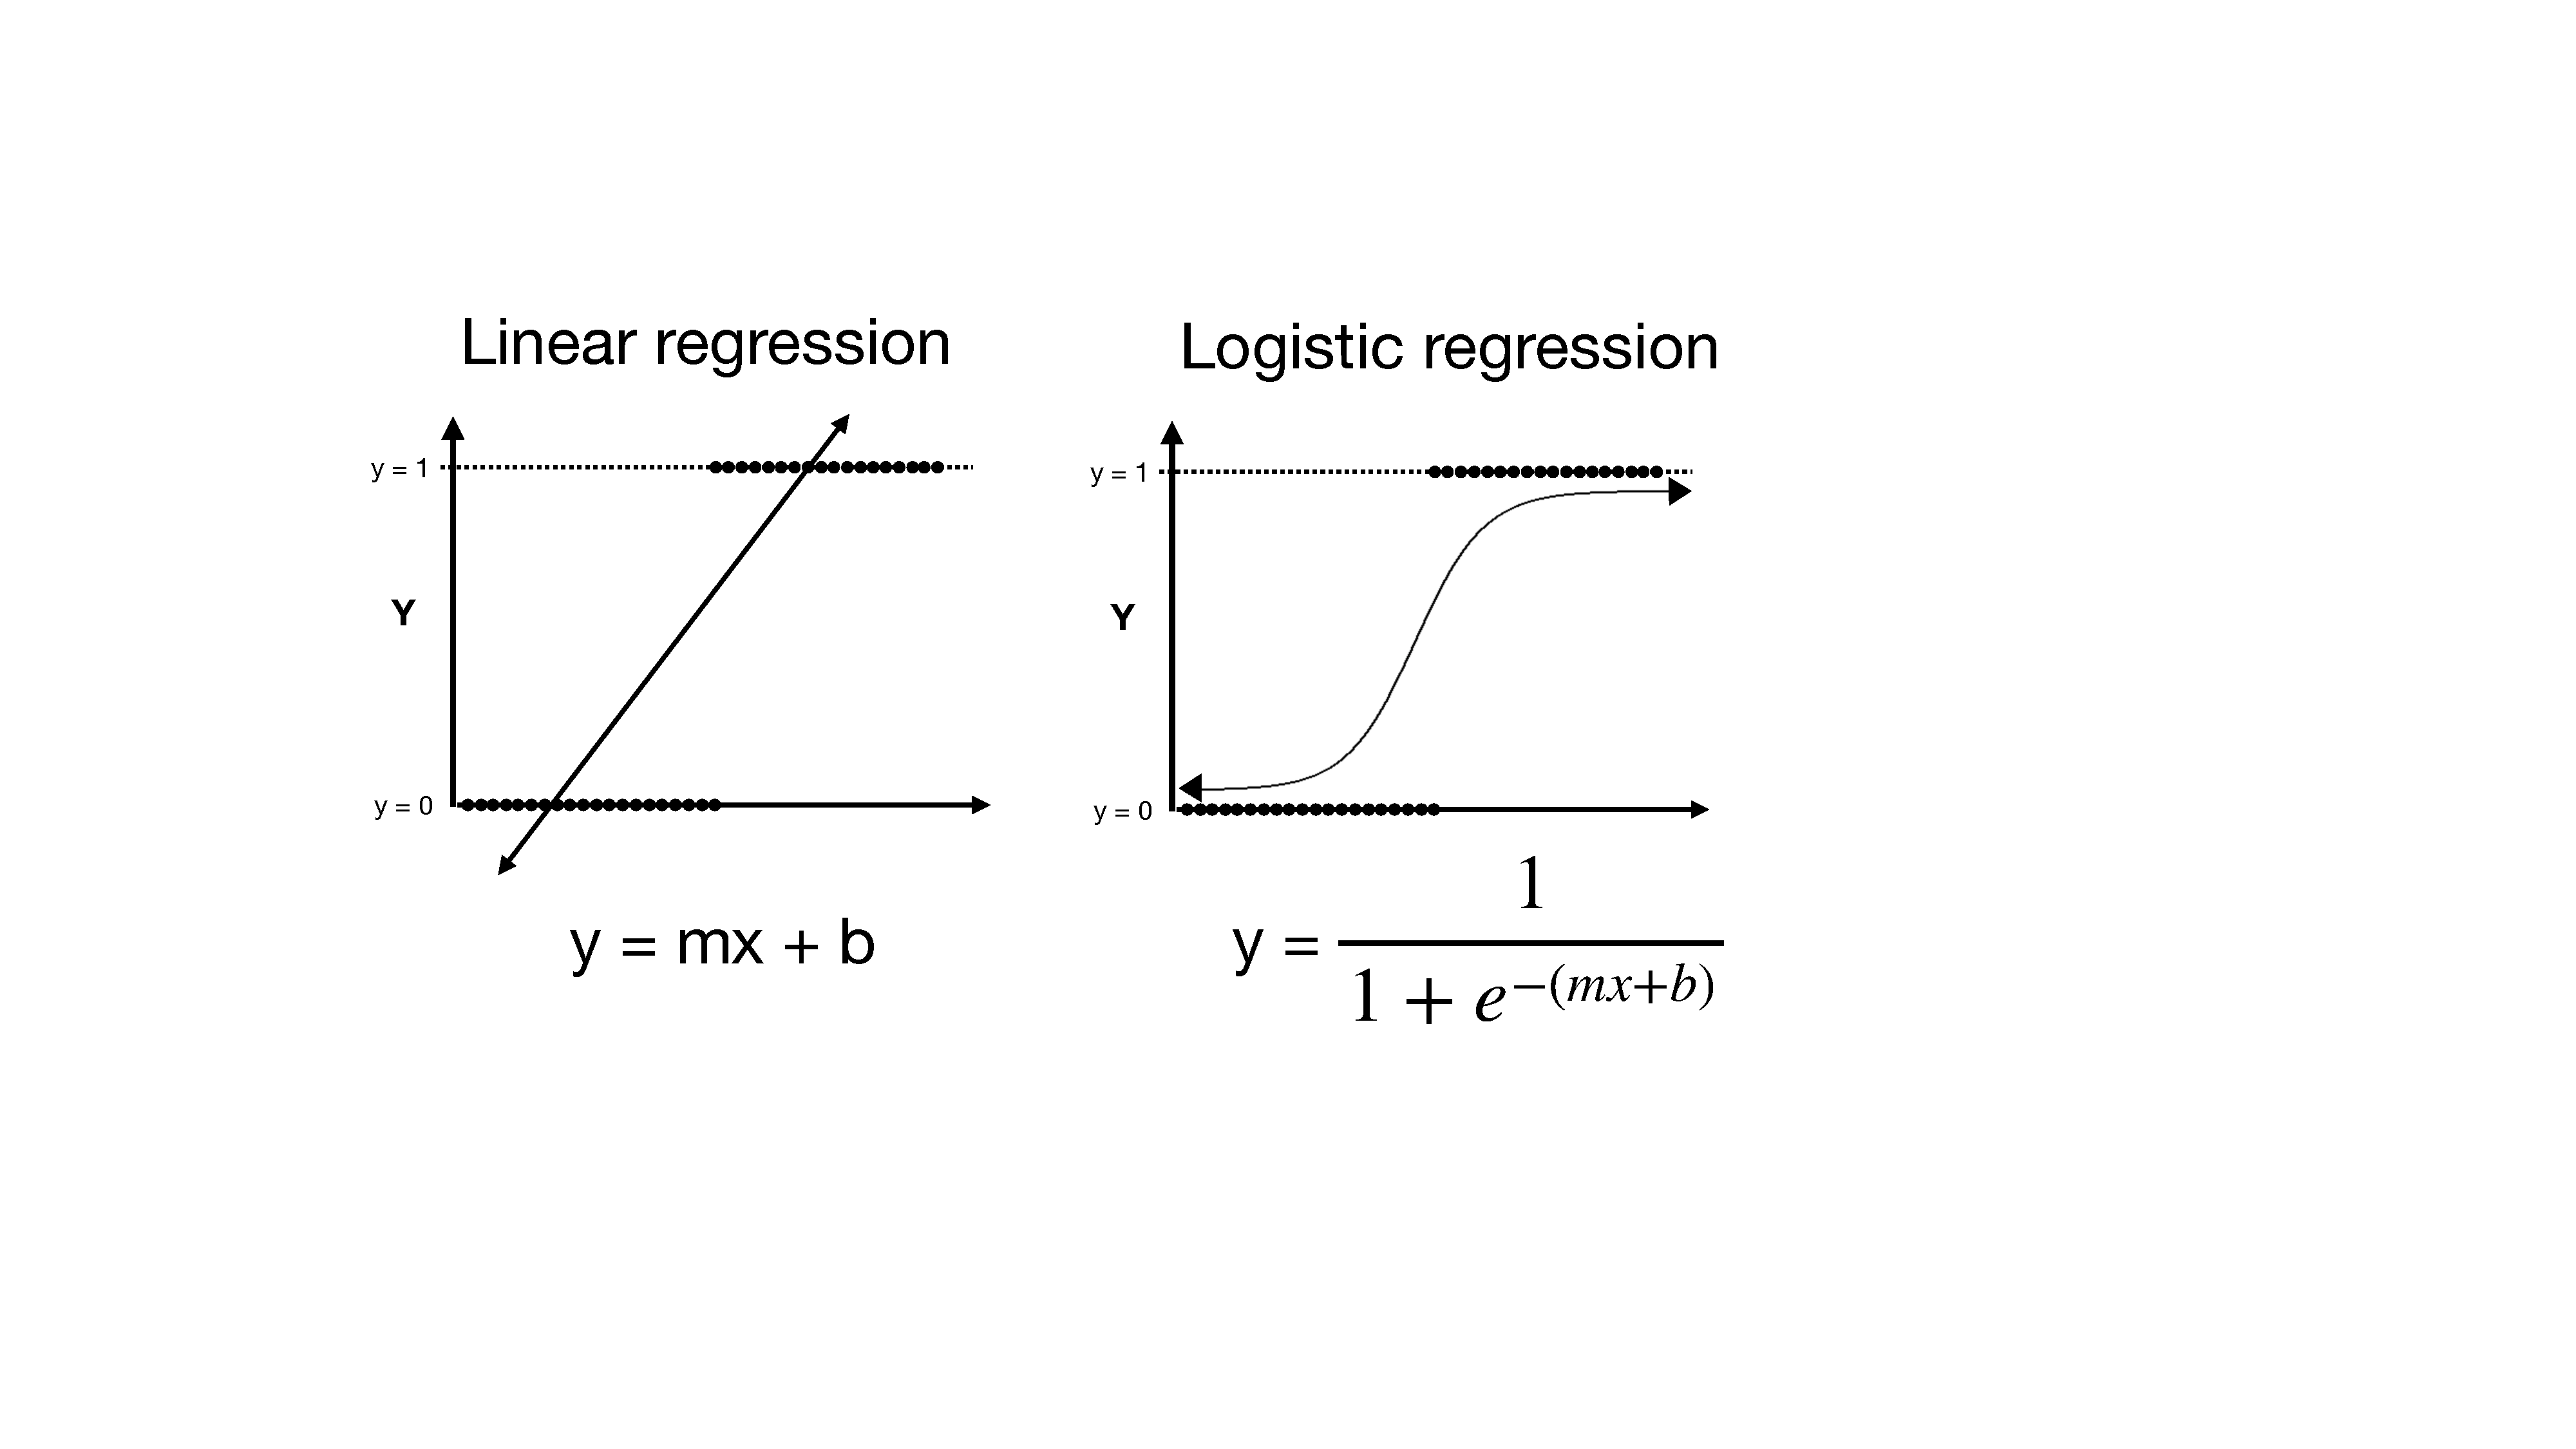
\includegraphics{figures/linear_vs_logistic.pdf}
      }
    }
    \only<2>{\resizebox{\textwidth}{!}{
        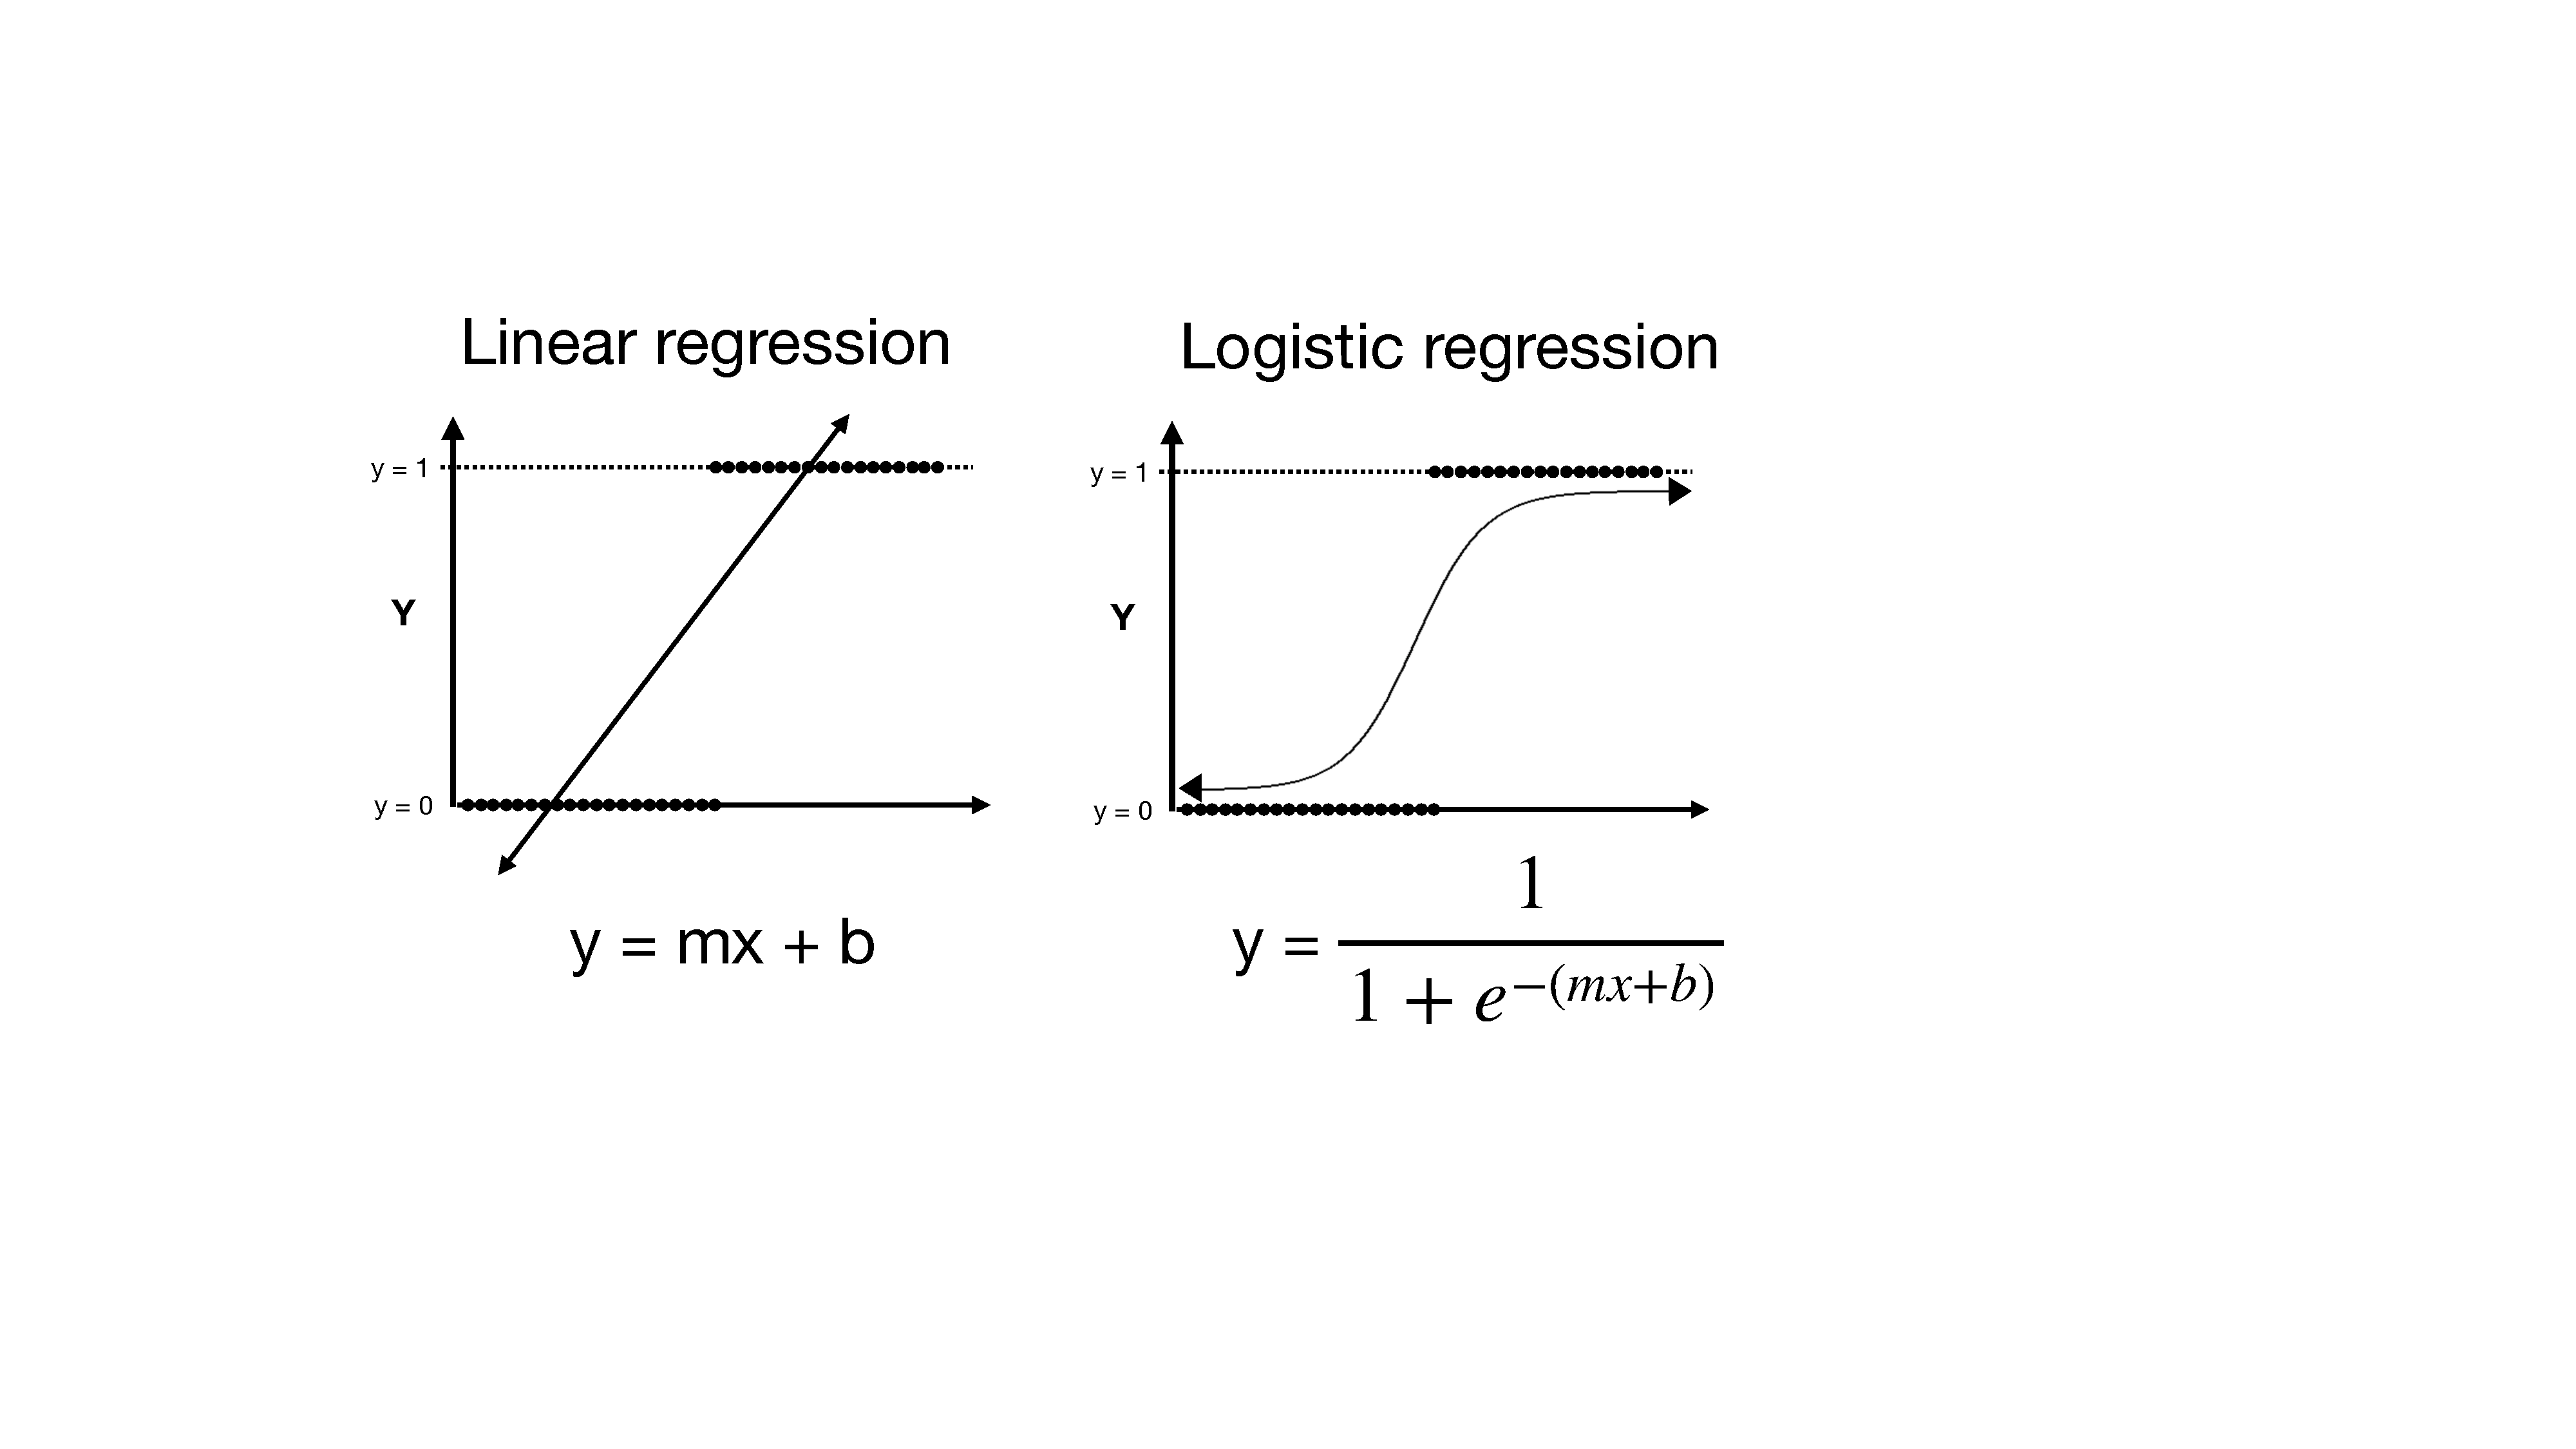
\includegraphics{figures/linear_vs_logistic.pdf}
      }
    }
    \only<3>{\resizebox{\textwidth}{!}{
        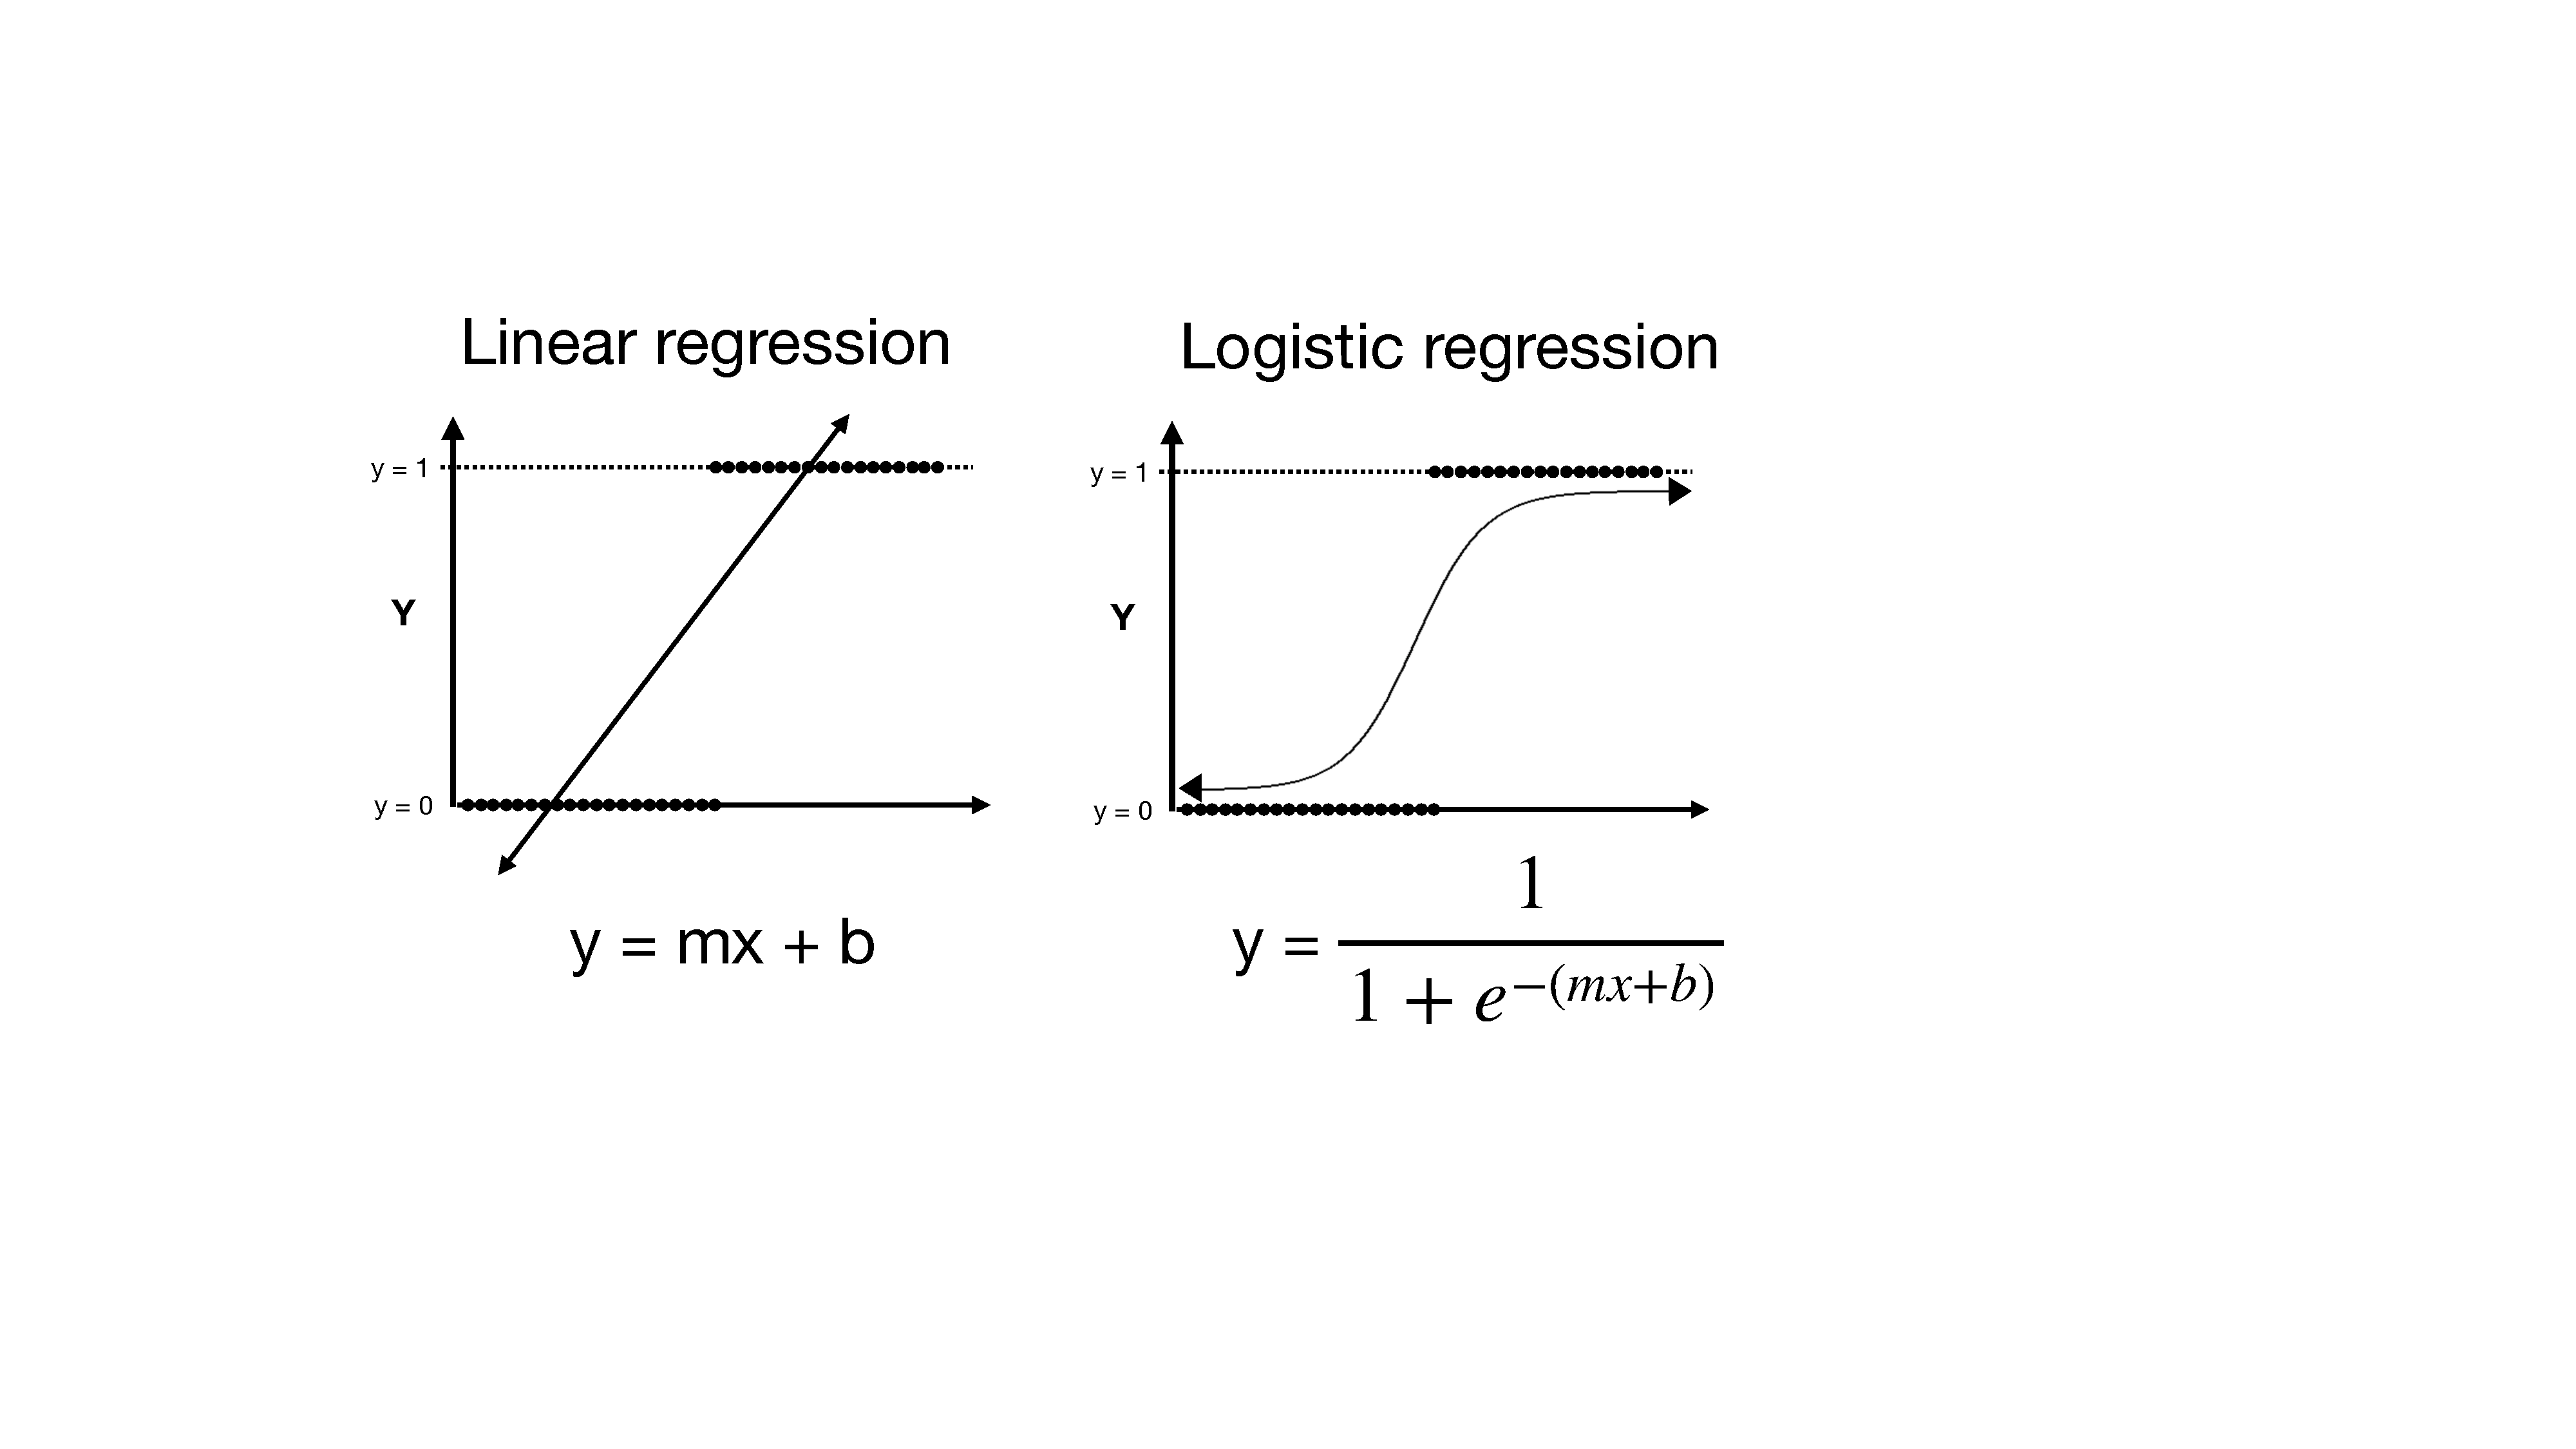
\includegraphics{figures/linear_vs_logistic.pdf}
      }
    }
  \end{column}
  \hfill
  \begin{column}{.4\textwidth}
    \footnotesize
    \begin{wideitemize}
    \item<1-> \textbf{Linear regression} for binary target variable will have a
      hard time try to come up with a best fit line that makes any sense.
    \item<2-> It'll try to fit a line that fits all of the data and it will end
      up predicting negative values and values over one, which is impossible.
    \item<3-> \textbf{Logistic regression} is built off of a logistic or sigmoid
      curve (S shape) and will always be between zero and one, which makes it a
      better fit for a binary classification problem.
    \end{wideitemize}
    \end{column}
  \end{columns}
\end{frame}


\begin{frame}[fragile]{\textbf{Q. When should you consider using Logistic Regression?}}
  \begin{wideitemize}
  \item \textbf{When to use?} Consider using it any time you
  \begin{wideitemize}\setlength{\itemsep}{0.6em}
  \item[-] You have a binary target variable.
  \item[-] You're interested in feature importance or having a better understanding
  of what's going on within the algorithm.
  \item[-] You have well-behaved\footnote{e.g., no many outliers, no many missing
  values, no complex relationships} data, need a \textbf{quick} initial benchmark.
  \end{wideitemize}
  \item \textbf{When not to use?} Consider not using it any time you
  \begin{wideitemize}\setlength{\itemsep}{0.6em}
  \item[-] You have a continuous target variable.
  \item[-] You have a massive amount of data\footnote{e.g., lots of features and
  very few rows, or lots of rows and very few features}.
  \item[-] You have unwieldy\footnote{e.g., many outliers, many missing
  values, complex relationships} data, performance\footnote{will usually do pretty
  well on any given problem, but will rarely be the best.} is the only thing that matters.
  \end{wideitemize}
  \end{wideitemize}
\end{frame}

% \begin{frame}[fragile]{\textbf{Q. What is the general form of multiple regression?}}
%   \begin{wideitemize}
%     \item The general form of the equation for linear regression.
%   \end{wideitemize}
% \end{frame}

\subsection{Clustering}
\begin{transitionsubframe}
  \begin{center}
    \Huge KMeans Clustering Algorithm
  \end{center}
\end{transitionsubframe}


\begin{frame}[fragile]{\textbf{Q. What is KMeans?}}
  \begin{wideitemize}
  \item \textbf{KMeans} is a unsupervised ML algorithm. It takes some data
    points as input and groups\footnote{grouping is the training phase of KMeans,
      and uses the square of the L2 norm as its cost function} them into $k$
    clusters\footnote{It uses the distance between points as a measure of
      similarity, based on $k$ averages (i.e. means).} (the output).\medskip
  \begin{wideitemize}
    \item This $k$ is called a hyper-parameter; a variable whose value we set
      before training.
    \item The idea is simple: You have a bunch of vectors $\in {\Bbb R}^{d}$.
      Then you init a bunch seed-guesses for the $k$ centers (centroids) of the
      clusters. You assign each vector to the nearest cluster. And then, when
      everything is done, you calculate the mean values of the clusters (updated $k$
      centers). And then you just do it again: you re-assign the nearest mean. Then
      you keep on going until it converges\footnote{Once those centroids stop
        moving(no further change in cost), the algorithm stop}.
  \end{wideitemize}
  \end{wideitemize}
\end{frame}

\begin{frame}[fragile]{\textbf{Q. When to use KMeans?}}
  \vspace{.4em}
  \begin{wideitemize}
    \item \textbf{When to use it}
    \begin{wideitemize}
      \item You have unlabeled data and don't know the number of clusters within it.
      \item You a have a decently large data set (less than 10K) with
      a smaller number of dimensions, these data are numeric, or continuous.
    \end{wideitemize}
    \item \textbf{When not to use it}
    \begin{wideitemize}
      \item High dimensional data, or data of varying sizes and density.
      \item Messy data with lots of outliers (as it can centroids can be dragged by outliers).
    \end{wideitemize}
  \end{wideitemize}
\end{frame}

\note[itemize]{
\item The user has to specify $k$ (the number of clusters) in the beginning
\item k-means can only handle numerical data
\item k-means assumes that we deal with spherical clusters and that each cluster
has roughly equal numbers of observations
}


\subsection{Naive Bayes}
\begin{transitionsubframe}
  \begin{center}
    \Huge Naive Bayes Classifier
  \end{center}
\end{transitionsubframe}


\begin{frame}[fragile]{\textbf{Q. What is Naive Bayes?}}
  \begin{wideitemize}
  \item \textbf{Naive Bayes} is a classification technique (Generative model) based
    on \textbf{Bayes Theorem} with an assumption of independence among predictors (features).
    In other words, a Naive Bayes classifier assumes that the presence of a particular feature in a
    class is unrelated to the presence of any other feature.
  \item Some \textbf{benefits} include:\medskip
  \begin{wideitemize}
    \item It's \textit{easy to build} and particularly \textit{useful for very large data sets}.
    \item Along with \textit{simplicity}, it's is known to outperform even highly
      sophisticated classification methods (NB has better \textit{resilience to missing} data than SVM).
  \end{wideitemize}
  \end{wideitemize}
\end{frame}

\begin{frame}[fragile]{\textbf{Q. Bayes Theorem (Quick Overview)?}}
  \makebox[\linewidth][c]{
    \resizebox{.3\linewidth}{!}{
      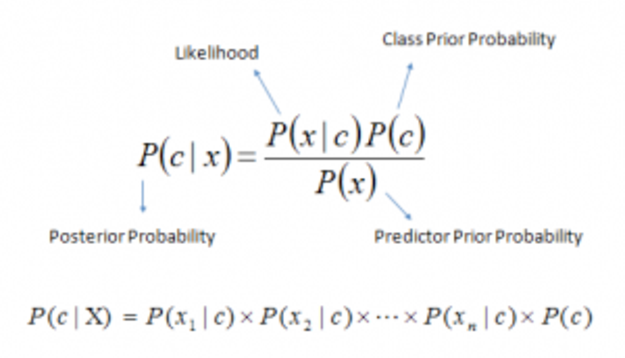
\includegraphics{figures/BayesTheorem.pdf}
    }
  }
  \begin{wideitemize}\small
  \item \textbf{Bayes theorem} \medskip
    \begin{wideitemize}\small
      \item Offers a way of calculating posterior probability $\Pr( c \mid x )$ from
      $\Pr( c )$, $\Pr( x )$, and $\Pr( x \mid c )$.
      \item $\Pr( c \mid x )$ simply means, ``given some feature vector $x_i \in X$, what is the
      probability of sample $i$ belonging to class $c_j \in C$?''
  \end{wideitemize}
  \end{wideitemize}

  \begin{framed}
    The \textbf{objective function} of \textbf{Naive Bayes}: Maximize $\Pr( C
    \mid X )$ given the training data to formulate a decision rule for new data.
  \end{framed}

\end{frame}


\begin{frame}[fragile]{\textbf{Q. How does Naive Bayes work?}}
  \begin{wideitemize}
  \item Step 1: Convert the data set into a frequency table (co-occurance matrix)
  \item Step 2: Create Likelihood table by finding the probabilities like
    ``Spam'' probability ($0.29$) and probability of ``No Spam'' ($0.64$).
  \item Step 3: Now, use Naive Bayesian equation to calculate the posterior
    probability for each class. The class with the highest posterior probability
    is the outcome of prediction.
  \end{wideitemize}
\end{frame}

\begin{frame}[fragile]{\textbf{Q. Example: Naive Bayes?}}
  \begin{wideitemize}
  \item \textbf{Problem:} Players will play if weather is sunny. Is this statement is correct?\medskip
    \begin{wideitemize}
    \item We can solve it using above discussed method of posterior probability.
    \item $\Pr( Y \mid \text{Sunny} ) = \Pr( \text{Sunny} \mid Y ) * \Pr( Y ) /
      \Pr( \text{Sunny} )$
    \item Here we have $\Pr( \text{Sunny} \mid Y ) = 3/9 = 0.33$, $\Pr( Y ) =
      9/14 = 0.64$, $\Pr( \text{Sunny} = 5/14 = 0.36$
    \item Now, $\Pr( Y \mid \text{Sunny} ) = 0.33 * 0.64 / 0.36 = 0.60$, which
      has higher probability.
    \end{wideitemize}
  \item Naive Bayes uses a similar method to predict the probability of
    different class based on various attributes. This algorithm is mostly used
    in text classification and with problems having multiple classes.
  \end{wideitemize}
\end{frame}


\end{document}
